\documentclass[11pt]{article}

\usepackage[margin=1in]{geometry}
\usepackage{amsmath}          % MUST precede newtxmath
\usepackage{amsthm}
\usepackage{graphicx}
\usepackage{booktabs}
\usepackage{subcaption}
\usepackage{xcolor}
\usepackage{mathtools}
\usepackage{float}
\usepackage{algorithm}
\usepackage{algpseudocode}
\usepackage{tikz}
\usetikzlibrary{shapes.geometric,arrows.meta,positioning,calc,fit,backgrounds}
\usepackage[colorlinks=true,linkcolor=blue,citecolor=blue,urlcolor=blue]{hyperref}

% ---- flowchart styles ------------------------------------------------- %
\tikzset{
  blk/.style={rectangle,rounded corners=2pt,draw=black!65,fill=blue!5,
              align=center,inner sep=4pt,minimum height=8mm,font=\footnotesize,
              text width=52mm},
  sml/.style={blk,text width=44mm},
  dec/.style={diamond,aspect=2.2,draw=black!65,fill=orange!12,align=center,
              inner sep=1pt,font=\footnotesize,text width=26mm},
  post/.style={blk,fill=green!6},
  ar/.style={-{Latex[length=2mm]},draw=black!70},
  fb/.style={-{Latex[length=2mm]},draw=black!70,dashed},
}

\newtheorem{proposition}{Proposition}
\newtheorem{remark}{Remark}

% ---- notation --------------------------------------------------------- %
% NOTE: these are defined with \providecommand+\renewcommand, NOT \newcommand.
% Short names like \T, \HH, \ii and \Real are defined by some packages/engines
% (\T is a text accent in several).  With \newcommand a pre-existing definition
% makes the declaration FAIL while silently keeping the old meaning, and every
% later use in math mode then raises "Missing $ inserted" far from the cause --
% a failure that appears on MiKTeX but not on TeX Live, or vice versa.
% \providecommand+\renewcommand always installs our meaning.
\makeatletter
\newcommand{\DefN}[2]{\@ifundefined{\expandafter\@gobble\string#1}{}{%
    \PackageInfo{notation}{overriding pre-existing \string#1}}%
  \providecommand#1{}\renewcommand#1{#2}}
\makeatother
% The \DefN applications are made AFTER the font packages (below), because
% newtxmath ALSO defines short names like \vv and would otherwise clobber our
% \renewcommand meanings if it loaded after them.

% ---- fonts -------------------------------------------------------------- %
% Palatino TEXT and MATHS via mathpazo.  (newpxtext/newpxmath were requested but
% are not installed and cannot be added -- the local TeX Live 2023 predates the
% remote 2026 repository, so tlmgr refuses the cross-release install.  mathpazo is
% the installed Palatino equivalent.)  Unlike newpxmath, mathpazo does NOT provide
% the AMS symbols, so amssymb IS required alongside it.
\usepackage{mathpazo}
\usepackage{amssymb}
\usepackage{bm}
\usepackage[scr=rsfso]{mathalfa}

%\usepackage{kpfonts}
%\usepackage[T1]{fontenc}
% ---- notation (applied AFTER the fonts so our meanings beat newtxmath) --- %
\DefN{\vth}{\bm{\theta}}
\DefN{\vu}{\mathbf{u}}
\DefN{\vv}{\mathbf{v}}
\DefN{\vn}{\mathbf{n}}
\DefN{\vx}{\mathbf{x}}
\DefN{\vU}{\mathsf{U}}
\DefN{\vb}{\mathsf{b}}
\DefN{\veps}{\bm{\varepsilon}}
\DefN{\rmd}{\,\mathrm{d}}
\DefN{\ii}{\mathrm{i}}
\DefN{\T}{^{\mathsf{T}}}
\DefN{\HH}{^{\mathsf{H}}}
\DefN{\Real}{\operatorname{Re}}
\DefN{\Imag}{\operatorname{Im}}
% Shared result numbers: \input by BOTH the paper and the slides so a
% number can never be updated in one and stale in the other.
% curl-constraint result numbers (set from examples/dolfinx_lens.py curl)
\DefN{\CURLU}{6.3}
\DefN{\CURLC}{2.8}
\DefN{\GAINU}{47}
\DefN{\GAINC}{12}
% through-hole lens numbers (examples/dolfinx_lens.py hole)  -- TO FILL
\DefN{\HGAINU}{49}
\DefN{\HCURLU}{5.7}
\DefN{\HGAINC}{17}
\DefN{\HCURLC}{3.55}
\DefN{\HRINV}{3.57}
% through-hole cloak numbers (examples/dolfinx_cloak_soft.py curl) -- TO FILL
\DefN{\CKREDU}{31}
\DefN{\CKCURLU}{3.4}
\DefN{\CKREDC}{21}
\DefN{\CKCURLC}{1.7}
\DefN{\CKZALL}{1.72}
% asymmetric through-hole lens (examples/dolfinx_lens.py holeasym) -- TO FILL
\DefN{\AGAIN}{50}
\DefN{\ACURL}{4.24}
\DefN{\ALIM}{4.17}
% curved energy routing / joint protection (examples/dolfinx_guide_joint.py)
\DefN{\GEXIT}{698}    % exit-port energy gain
\DefN{\GGUARD}{0.17}   % guard-annulus energy ratio (<1 is good)
\DefN{\GPROT}{4002}    % protection factor (exit/guard ratio improvement)
\DefN{\GRATZ}{127}    % baseline guard/exit ratio
\DefN{\GZ}{6.59}       % max|zeta| of the reported design
\DefN{\GZALL}{6.67}  % 1/R_TOW (print head), NOT 1/R_J
\DefN{\GCONFZ}{22}   % downstream confinement, baseline
\DefN{\GCONFO}{97}   % downstream confinement, optimized
% multi-target beam shaping (examples/dolfinx_lens.py multi) -- TO FILL
\DefN{\MCONA}{2}
\DefN{\MCONB}{19}
\DefN{\MTGAIN}{19}
\DefN{\MCIMP}{10}
% flat-band metamaterial (examples/flatband_demo.py) -- TO FILL
\DefN{\FBBAND}{3}
\DefN{\FBWZ}{2.78}
\DefN{\FBWO}{0.59}
\DefN{\FBFLAT}{4.7}
\DefN{\FBGU}{+0.42}
\DefN{\FBGD}{+0.66}
\DefN{\FBWV}{0.65}
\DefN{\FBGUV}{+0.41}
\DefN{\FBGDV}{+0.67}
% multi-functional metamaterial (examples/multifunc_demo.py) -- co-design sweep
\DefN{\MFSTIFFGAIN}{61} % percent stiffness advantage at equal gap-open status
\DefN{\MFGAPX}{19}      % gap ratio
\DefN{\MFPARLO}{+0.84}  % parity of the lower gap-edge mode at Gamma

% ---- topological valley guiding (examples/valley_*.py) ----------------- %
% bulk complete gap, conforming cell, 41x41 BZ sampling (converged)
\DefN{\VGAPLO}{7.014}
\DefN{\VGAPHI}{7.567}
\DefN{\VGAPW}{0.553}
% ribbon wall-localized branch: upper end -> protected window [VGAPLO, VKINKHI]
\DefN{\VKINKHI}{7.27}
\DefN{\VWCONF}{0.95}      % wall confinement in the protected window
\DefN{\VWCONFB}{0.51}     % ... below the gap
% mesh-convergence of in-gap transmission (h = 0.12, 0.09, 0.06)
\DefN{\VCONVC}{1.9}       % conforming: spread factor over h
\DefN{\VCONVP}{590}       % painted:    spread factor over h
\DefN{\VRODOFF}{2.9}      % painted per-rod centroid offset, % of R
% robustness at omega = 7.2 (inside the protected window), conforming h=0.09
\DefN{\VROMEGA}{7.2}
\DefN{\VRPRIS}{0.65}      % pristine transmission
\DefN{\VRVAC}{21}         % vacancy, % of pristine
\DefN{\VRDIS}{38}         % orientation disorder, % of pristine
\DefN{\VRCON}{5400}       % pristine in-band / out-of-band contrast
% ---- finite truncated panel (examples/multifunc_finite.py) ------------- %
\DefN{\FPGAPCO}{0.632}    % co-design complete gap
\DefN{\FPGAPGE}{0.319}    % geometry-only complete gap
\DefN{\FPCCO}{4.80}       % co-design C_bulk
\DefN{\FPCGE}{4.27}       % geometry-only C_bulk
\DefN{\FPKCO}{6.29}       % co-design panel static k_eff
\DefN{\FPKGE}{6.12}       % geometry-only panel static k_eff
\DefN{\FPILMEAN}{50}      % 6-period in-gap insertion loss, mean
\DefN{\FPILPEAK}{55}      % ... peak
\DefN{\FPKAPPA}{0.42}     % kappa*a per cell
\DefN{\FPDEC}{0.35}       % decades of isolation per cell
\DefN{\FPILTEN}{2158}      % insertion loss at 10 periods
\DefN{\FPCONCO}{5.37}     % in-own-gap contrast, co-design
\DefN{\FPCONGE}{4.46}     % in-own-gap contrast, geometry-only
\DefN{\FPBROAD}{9.0}      % geometry-only broadband transmission deficit
% ---- finite-panel as-built (crisp two-phase) check --------------------- %
\DefN{\FPABGAP}{0.669}   % as-built complete gap
\DefN{\FPABGAPD}{0.692}  % as-designed complete gap it is compared to
\DefN{\FPABPCT}{97}      % as-built gap as % of as-designed width
\DefN{\FPABIL}{32}       % as-built in-gap insertion loss
   % shared with the beamer slides


\title{\bfseries wavetopo --- companion notes: variants, periodic media, a modal bracket,
and valley-Hall guiding}
\author{Joshua R.~Tempelman}
\date{Working notes --- \today}
\graphicspath{{../}{../figs/}}
\begin{document}
\maketitle
\paragraph{Status of these notes.} These sections were split out of the main manuscript
(\texttt{dolfinx\_wave\_control.tex}), whose question is how much control fiber
orientation alone exerts on in-plane elastic waves, by what mechanism, and within what
limits. Each section below answers a \emph{different} question and is preserved
verbatim from the earlier draft, with its own caveats. Three caveats from the main
paper apply here. (i) Single-frequency focus-energy gains of finite plates include
resonant field build-up and must be decomposed into redirection and amplification
before they are compared. (ii) Single-frequency cloak reductions are narrowband.
(iii) The periodic band-gap claims are subject to the dense-$\mathbf k$ caveats stated
in the text.
\subsection{Multi-target beam shaping (two foci and a null)}
\label{sec:multi}
The same machinery handles a genuinely multi-objective goal by a signed region
weight. We ask the plate to \emph{maximize} energy in two separated focus regions
while \emph{minimizing} it in a third between them: setting $w=+1$ on the two
targets and $w=-\lambda$ on the null ($\lambda=1$) and maximizing
$J=\int_\Omega w|\vu|^2$ drives a fiber beam splitter. The straight-fiber baseline
illuminates the three regions almost equally (target/null contrast $\MCONA$); the
optimized orientation splits the wave into the two off-axis foci and holds the
centre as a local dark node, raising the target/null contrast to $\MCONB$ while
the foci-to-null energy swing against the baseline reaches
$\MTGAIN\times$ (Figure~\ref{fig:multi}). (The whole field amplifies off the very
dim straight-fiber baseline, so the meaningful measure of the null is its
\emph{contrast} against the neighbouring foci, not its absolute level.) Only the
signed objective changed --- the physics, adjoint, parametrization and toolpath
pipeline are identical to the single-focus lens.

\begin{figure}[h]
\centering
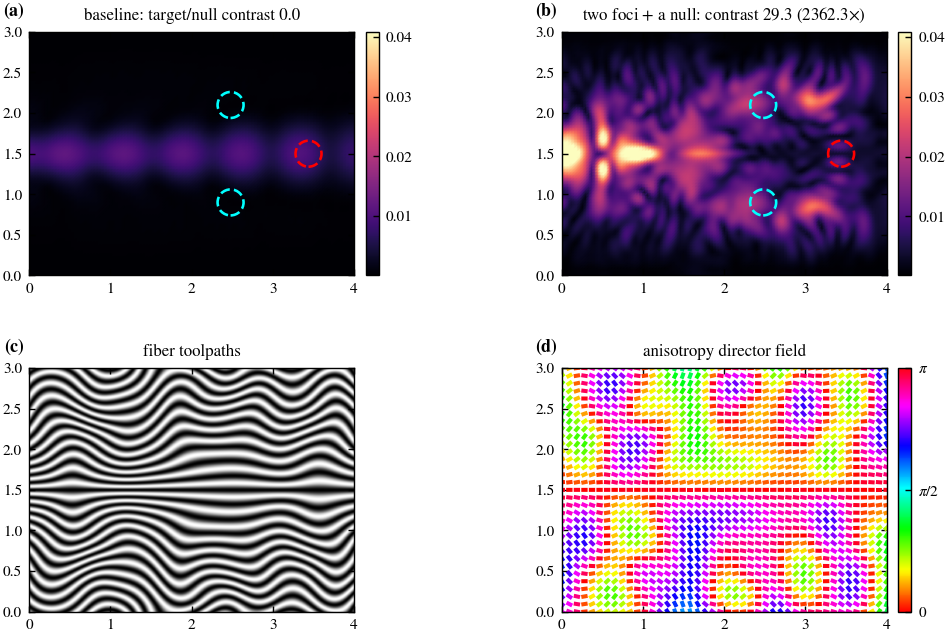
\includegraphics[width=0.99\textwidth]{figs/dfx_lens_multi.png}
\caption{Multi-target beam shaping. The objective maximizes energy in the two
targets (cyan) and minimizes it in the null (red). Top: straight-fiber baseline vs.\
the optimized two-focus-plus-null design (target/null contrast $\MCONA\to\MCONB$).
Bottom: the phase-field fiber toolpaths (a beam splitter) and the convergence of
$J$. Same solver, adjoint and parametrization as the single-focus lens; only the
signed region weight differs.}
\label{fig:multi}
\end{figure}

\section{Designing around prescribed through-holes}
\label{sec:hole}
The reference work ties the curvature limit directly to geometry: a
\emph{prescribed circular void} (a passive, zero-density through-hole) of radius
$R$ imposes a local minimum turning radius on the fibers wrapping it, so the
manufacturable curvature limit is $\zeta_{\rm all}=1/R$. We reproduce this rule in
both wave-control settings.

The holes enter the physics \emph{geometrically}: each disk is cut from the domain
with \texttt{gmsh}/OCC and the triangulation conforms to its boundary
(\S\ref{sec:spaces}, \texttt{wavetopo/dolfinx\_mesh.py}), so the rim is exactly
circular and traction-free through the natural boundary condition of the weak
form, with the element size halved on the rim where the diffraction happens. This
matters more than it may appear. The obvious alternative --- representing the hole
as a SIMP soft void ($z=0$, so $z^p\mathbf D_f\to0$) on a structured grid ---
replaces the circle by the set of elements whose centroid lies inside it. The
resulting boundary is a staircase that scatters off its own corners, concentrates
spurious energy on the rim, and defines the radius only to within one element:
precisely the radius $R$ that the curvature rule $\zeta_{\rm all}=1/R$ is tied to.
Conforming to the geometry is the substantive reason these problems are solved in
\texttt{dolfinx} rather than in the structured Q4 code used for the periodic cell
of \S\ref{sec:meta}, where (the geometry being the density field itself) there is
no boundary to conform to and a structured grid is the better tool.

\subsection{Wave lens with two circular through-holes}
\label{sec:lenshole}
We cut two symmetric circular through-holes ($R=0.28$, so $1/R\approx\HRINV$)
into the beam path of the lens and again maximize the focus energy. Without a
curvature limit the optimizer routes the fibers through the gap between the holes
and around their flanks, refocusing the diffracted field with a
$\HGAINU\times$ gain but at the cost of tight bends where the tows crowd past the
voids ($|\zeta|_{\max}=\HCURLU$). Imposing the through-hole limit
$|\zeta|\le1/R$ (Eq.~\eqref{eq:curl}) relaxes those bends to the radius of the
holes themselves: the peak curvature falls to $\HCURLC$, just inside the limit
$1/R=\HRINV$, and the gain settles at $\HGAINC\times$
(Figure~\ref{fig:lenshole}). The toolpaths now wrap the prescribed voids with arcs
no tighter than the holes --- a directly printable layout. Note that the
constrained design is \emph{feasible}, not merely penalized: the reported
$|\zeta|_{\max}$ lies below $\zeta_{\rm all}$ rather than near it from above.

\begin{figure}[h]
\centering
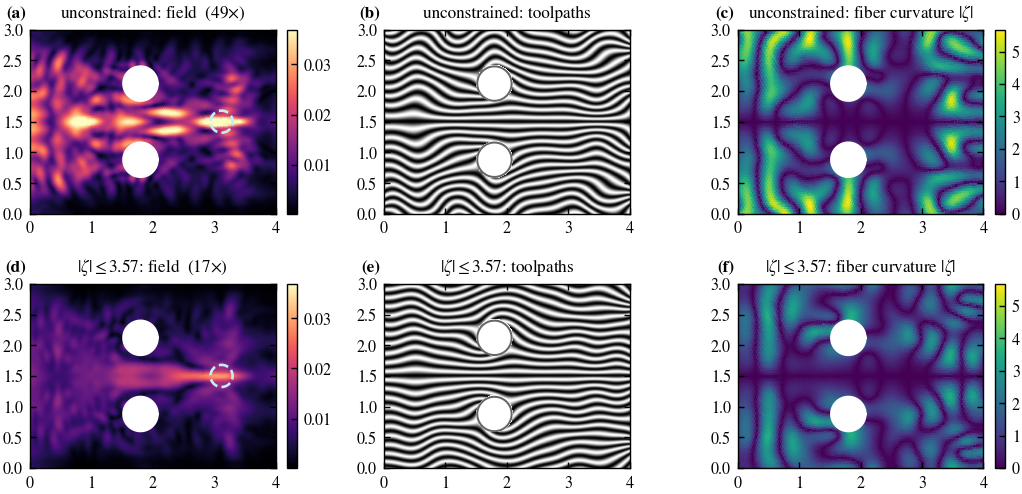
\includegraphics[width=0.99\textwidth]{figs/dfx_lens_hole.png}
\caption{Wave lens with two prescribed circular through-holes (white). Top row:
unconstrained --- the fibers route around the voids and refocus the wave, with
tight bends ($|\zeta|_{\max}=\HCURLU$). Bottom row: with the through-hole limit
$|\zeta|\le1/R\approx\HRINV$, the toolpaths wrap the holes with arcs no tighter
than the holes ($|\zeta|_{\max}=\HCURLC$) at a modest focus cost. Columns: field,
toolpaths, fiber-curvature $|\zeta|$ map. The dashed circle in the field panels
marks the focus target the lens is optimized to fill.}
\label{fig:lenshole}
\end{figure}

\subsection{Asymmetric through-holes: the design re-optimizes per geometry}
\label{sec:lenshole_asym}
The symmetric layout of Figure~\ref{fig:lenshole} could give the misleading
impression that the fiber field is fixed and only the holes move. It is not: the
orientation is re-optimized from scratch for each hole geometry. To make this
explicit we place two \emph{asymmetric} through-holes --- different centres and
radii, breaking the $y=L_y/2$ mirror symmetry --- and drop the symmetry constraint
on the design entirely (a plain, non-symmetric CS-RBF support grid). The optimizer
returns a visibly \emph{asymmetric} fiber field that threads the wave through the
off-centre gap between the voids and re-focuses on the target, a
$\AGAIN\times$ gain with peak curvature $|\zeta|_{\max}=\ACURL$
(Figure~\ref{fig:lenshole_asym}). Here the curvature limit is set by the
\emph{smaller} of the two holes, $\zeta_{\rm all}=1/0.24=\ALIM$, and we report
honestly that the converged design ends marginally \emph{above} it
($\ACURL$ vs.\ $\ALIM$, a $1.7\%$ overshoot): the constraint is imposed by the
smooth quadratic penalty of \S\ref{sec:curl} under continuation, which drives the
curvature down to the neighbourhood of the bound but does not enforce it exactly.
The symmetric case of \S\ref{sec:lenshole} does land strictly inside its bound
($\HCURLC$ vs.\ $\HRINV$); this one does not quite, and a hard constraint (or a
larger terminal $\mu$) would be required to certify feasibility. The toolpaths and the
director map wrap the two holes differently, exactly as the differing local
geometry demands --- the design is genuinely solved anew, not mirrored.

\begin{figure}[h]
\centering
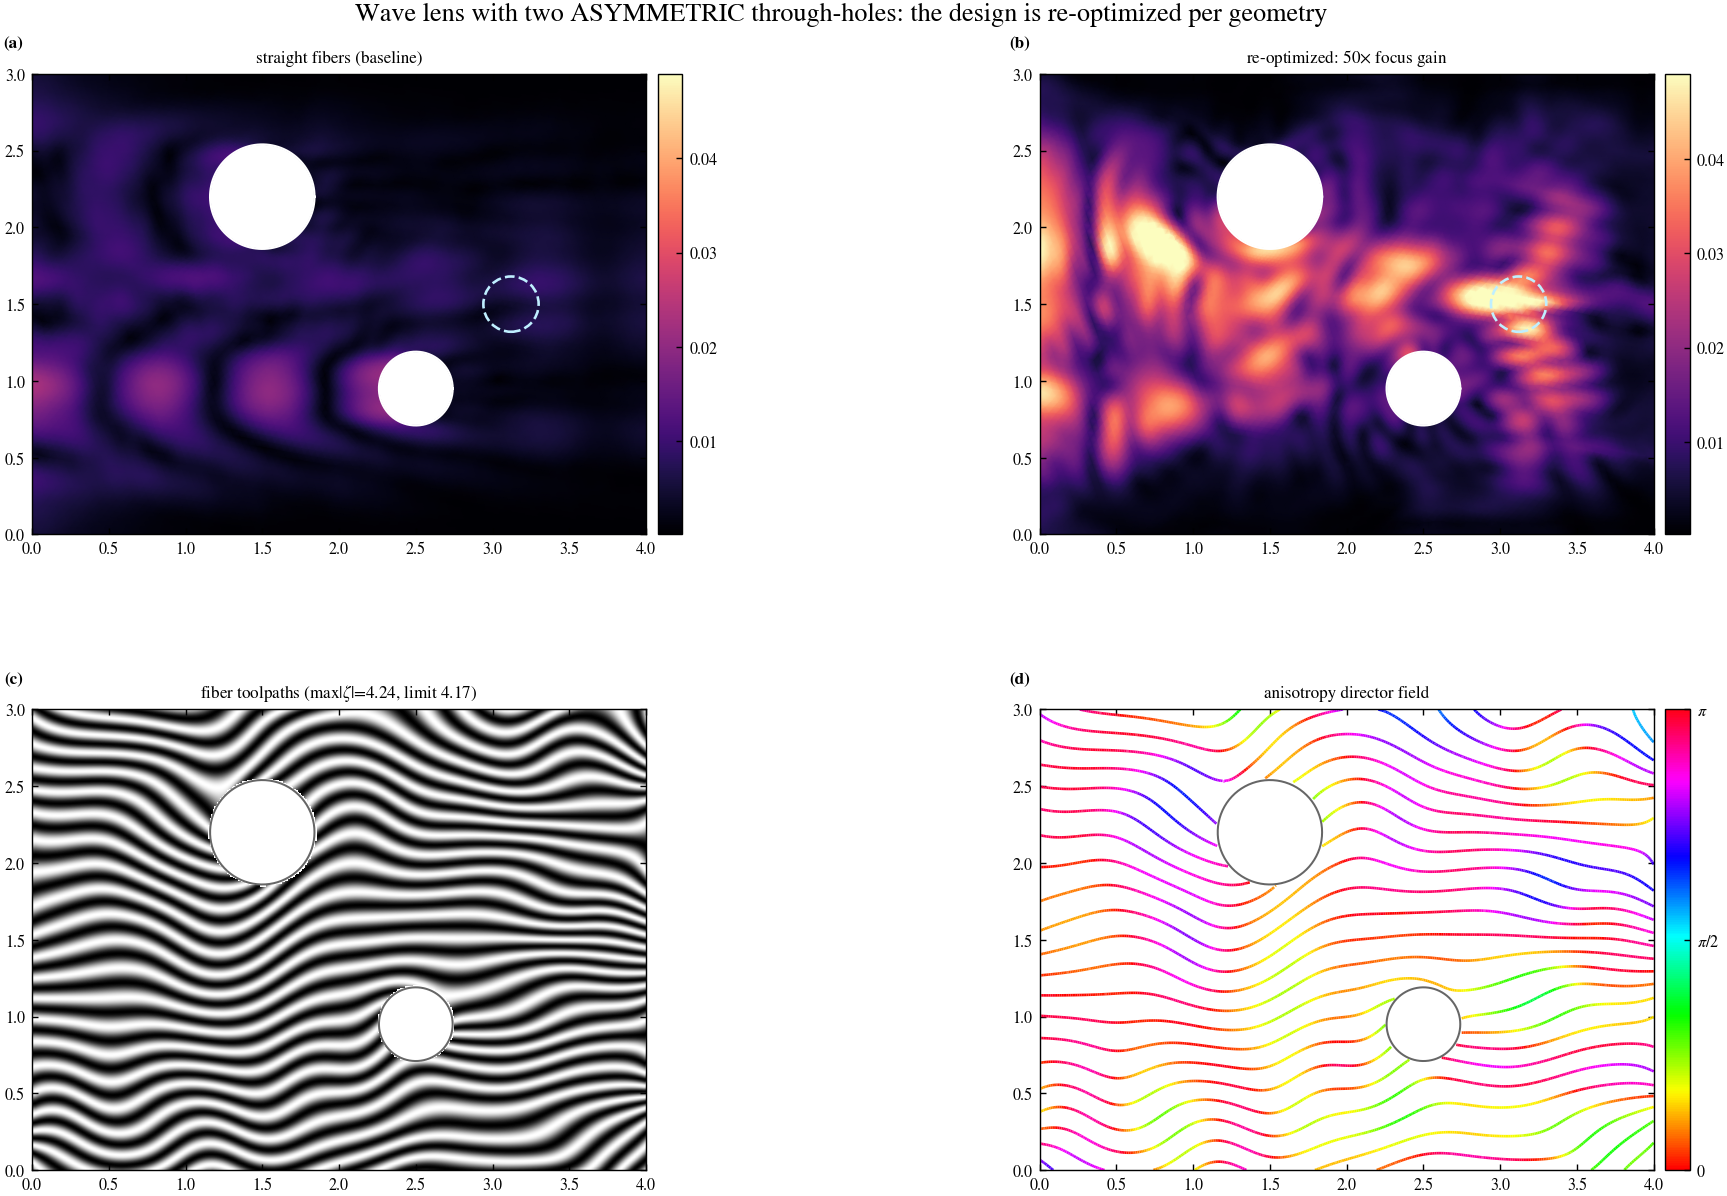
\includegraphics[width=0.99\textwidth]{figs/dfx_lens_hole_asym.png}
\caption{Wave lens with two \emph{asymmetric} through-holes (no symmetry imposed).
Top: straight-fiber baseline and the re-optimized field ($\AGAIN\times$ focus
gain). Bottom: the phase-field fiber toolpaths and the anisotropy director map ---
both asymmetric, wrapping the differently placed/sized voids as their local
geometry requires. This is a genuine per-geometry re-optimization, not a mirrored
copy of Figure~\ref{fig:lenshole}. The dashed circle in the field panels marks the
focus target.}
\label{fig:lenshole_asym}
\end{figure}

\subsection{Routing energy around a joint: a curved delivery corridor}
\label{sec:guide}
The through-hole studies so far treat the void as an obstacle to be worked around.
A bolt hole or a fastened joint is more than that: it is the place where a panel
\emph{fails}. Fatigue cracks nucleate at the rim, so vibrational energy
concentrating there is precisely what a designer wants to avoid. This suggests a
design problem the reference work does not pose --- route the energy along a
prescribed \emph{curved} path that detours around the joint, delivering it
downstream while keeping the fatigue-critical rim quiet.

We place the joint (radius $R_J=0.40$, cut conformally from the mesh) squarely on
the straight line between the drive and a delivery port, so the direct path is
blocked and the energy \emph{must} detour. Three regions define the goal: a curved
corridor whose centreline is a smooth bump lifting the path over the joint,
\begin{equation}
  y_c(x)=y_J+A\,e^{-((x-x_J)/s)^2},\qquad
  \Omega_{\rm cor}=\bigl\{\,|y-y_c(x)|<h\,\bigr\},
  \label{eq:corridor}
\end{equation}
an exit port $\Omega_{\rm exit}$ downstream of the joint, and a guard annulus
$\Omega_{\rm gd}=\{R_J\le r<R_J+g\}$ hugging the rim. Both objectives are carried
by a \emph{single signed} region weight, exactly the device used for the
multi-target lens,
\begin{equation}
  w(\vx)=\underbrace{\mathbb 1_{\Omega_{\rm cor}\cup\Omega_{\rm exit}}(\vx)}
         _{\text{deliver here}}
  \;-\;\lambda\underbrace{\mathbb 1_{\Omega_{\rm gd}}(\vx)}_{\text{protect here}},
  \qquad
  \max_{\hat\theta}\ J=\int_\Omega w\,|\vu|^2 ,
  \label{eq:guideobj}
\end{equation}
with $\lambda=2.5$. Note $J$ is genuinely \emph{signed} --- at the straight-fiber
baseline the guard term dominates and $J<0$ --- so this problem is descended with
the raw gradient rather than the log-objective of \S\ref{sec:adj}, which would be
undefined. The fiber curvature is limited to the joint's own radius,
$\zeta_{\rm all}=1/R_J=\GZALL$, so the tows may not bend tighter than the hole
they wrap.

The straight-fiber baseline illustrates the problem: the beam launched at the
aperture diffracts, spreads onto the joint, and barely reaches the port --- the
guard annulus carries $\GRATZ\times$ more energy than the exit, and only
$\GCONFZ\%$ of the downstream energy is in the corridor at all. Designing the
orientation alone raises the delivered energy by $\GEXIT\times$, cuts the guard
energy to $\GGUARD$ of baseline, and lifts the downstream confinement from
$\GCONFZ\%$ to $\mathbf{\GCONFO\%}$: the field becomes a continuous ribbon that
tracks the corridor over the joint and terminates at the port
(Figure~\ref{fig:guide}). The design is feasible, $|\zeta|_{\max}=\GZ$ against the
print-head limit $\GZALL$.

\paragraph{Three modelling choices decide whether this works at all.} Each was
arrived at by a failure, and each is worth stating because the failures are silent
--- they return healthy-looking headline numbers for designs that do the wrong
thing.

\emph{(i) The source must be localized.} With a full-width plane-wave drive most
of the field never enters the corridor, so there is nothing to channel and the
result is a diffraction pattern with a bright spot at the port. A narrow aperture
at the channel mouth is what makes the problem a guiding problem.

\emph{(ii) The curvature limit must be the print head's, not the hole's.} Setting
$\zeta_{\rm all}=1/R_J$ --- the reference work's rule for fibers \emph{wrapping} a
prescribed void --- is the wrong constraint for a guiding channel and is strictly
binding: the optimizer sits pinned at the bound with the trust region collapsed
and the objective still negative. The physically relevant limit is the machine's
minimum turning radius, here $\zeta_{\rm all}=1/R_{\rm tow}=\GZALL$; the converged
design uses $\GZ$, i.e.\ nearly three times the curvature the hole rule would have
allowed.

\emph{(iii) The delivery reward must saturate.} With a reward linear in
$E_{\rm exit}/E_{\rm exit}^0$ the delivered energy reaches $6300\times$ baseline,
so that single term contributes $6300$ against a guard penalty of $8$ --- a
$760\!:\!1$ imbalance --- and the optimizer buys delivery by letting the joint get
$20\times$ \emph{busier}, defeating the purpose. A logarithmic reward
($\log 6300=8.7$) has diminishing returns, so protecting the rim remains worth
doing however bright the port already is. The gradient still costs one adjoint
solve: for $J=\sum_k c_k E_k$ the adjoint weight is $\sum_k(\partial J/\partial
E_k)\,w_k$, with $\partial J/\partial E_{\rm exit}=W_E/E_{\rm exit}$ re-evaluated
at the current iterate.

\paragraph{Confinement is bought by the leakage penalty, and it has an optimum.}
Table~\ref{tab:guidetrade} sweeps $\lambda_{\rm out}$. Too weak and the wave
diffracts around \emph{both} sides of the joint --- a physically natural but
undirected split, with barely half the downstream energy in the corridor. Too
strong and the optimizer suppresses the field rather than steering it: delivery
collapses by more than an order of magnitude while confinement also falls, since a
suppressed field is not a guided one. The intermediate value dominates the whole
sweep on every metric simultaneously.

\begin{table}[h]
\centering\small
\caption{Effect of the leakage penalty $\lambda_{\rm out}$ on the joint-routing
design (all other parameters fixed). Exit gain and guard ratio are relative to the
straight-fiber baseline; a guard ratio below one means the fatigue-critical
annulus is quieter than baseline. ``Confinement'' is the fraction of downstream
($x>x_J$) interior energy lying inside the corridor, which at the baseline is
$\GCONFZ\%$.}
\label{tab:guidetrade}
\begin{tabular}{ccccc}
\toprule
$\lambda_{\rm out}$ & exit gain & guard ratio & protection & confinement\\
\midrule
$0.25$ & $426\times$ & $0.13$ & $3218\times$ & $45\%$\\
$\mathbf{0.80}$ & $\mathbf{698\times}$ & $\mathbf{0.17}$ & $\mathbf{4002\times}$
  & $\mathbf{97\%}$\\
$2.0$  & $339\times$ & $0.15$ & $2303\times$ & $99.9\%$\\
$5.0$  & $29\times$  & $0.29$ & $99\times$   & $86\%$\\
\bottomrule
\end{tabular}
\end{table}

\begin{figure}[h]
\centering
\IfFileExists{figs/dfx_guide_joint.png}
  {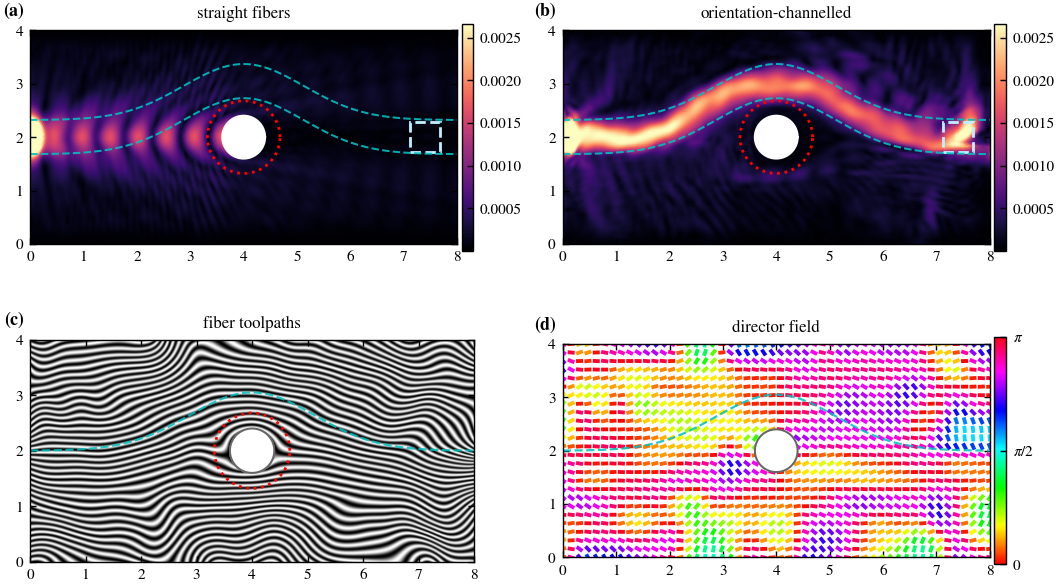
\includegraphics[width=0.99\textwidth]{figs/dfx_guide_joint.png}}
  {\fbox{\parbox[c][35mm][c]{0.9\textwidth}{\centering\itshape
   figure pending: run in progress}}}
\caption{Routing elastic energy along a curved corridor around a through-hole
joint. Top: the straight-fiber baseline, where energy concentrates on the joint,
versus the orientation-guided design, which threads the wave along the corridor
(cyan dashed) and into the exit port (light dashed box) while keeping the
fatigue-critical guard annulus (red dotted) quiet. The joint is cut from the
geometry, so its rim is exactly circular and traction-free. Bottom: the phase-field
fiber toolpaths, which arc over the joint within the curvature limit
$|\zeta|\le1/R_J$, and the anisotropy director map. Only the fiber orientation is
designed.}
\label{fig:guide}
\end{figure}

\section{Periodic metamaterials: co-designed flat bands and band gaps}
\label{sec:meta}
The wave-control problems above steer a wave through a finite plate. The same
orthotropic fiber design also shapes the intrinsic \emph{dispersion} of a periodic
fiber-composite metamaterial. Here we co-design \emph{two} fields on a single
periodic unit cell --- the density $z$ (topology) and the fiber orientation
$\theta$ (toolpath) --- to make a chosen band \emph{flat} (a slow-wave,
high-density-of-states mode) and \emph{isolated} by gaps to its neighbours. The
constitutive model is identical to \S\ref{sec:model} (the rotated orthotropic
$\mathbf D_f(\theta)$ with SIMP density), but the solver is a different one.

\begin{remark}[Two independent solvers]
\label{rem:solvers}
The results of \S\ref{sec:results}--\S\ref{sec:hole} are computed in
\texttt{dolfinx}/\texttt{FEniCSx} on an unstructured triangulation with
\texttt{PETSc} linear algebra and UFL-generated adjoints
(\texttt{wavetopo/dolfinx\_wave.py}). The band-structure results of this section are
\emph{not}: they come from an independent, self-contained
\texttt{numpy}/\texttt{scipy} Q4 quadrilateral code
(\texttt{wavetopo/cfrp.py}$\rightarrow$\texttt{wavetopo/bloch.py}) that imports no
\texttt{dolfinx}, \texttt{UFL}, \texttt{PETSc} or \texttt{SLEPc}. Bloch
periodicity is imposed by an explicitly constructed complex reduction matrix
$\mathbf T(\mathbf k)$, and \eqref{eq:bloch} is solved as a \emph{dense} Hermitian
generalized eigenproblem (\texttt{scipy.linalg.eigh} on a band subset) --- which is
why the per-$\mathbf k$ cost grows steeply with mesh size
(Table~\ref{tab:sweep}). The two codes therefore share the \emph{physics} (the same
$\mathbf Q_f$, the same $\mathbf D_f(\theta)=\mathbf T\mathbf Q_f\mathbf T\T$, the
same SIMP interpolation) and the same design machinery (CS-RBF map, density
filter, MMA), but no assembly or linear-algebra code whatsoever. That independence
is worth stating plainly rather than eliding: each implementation is a check on the
other's constitutive algebra, and neither set of results inherits a bug from the
other.
\end{remark}

\subsection{Bloch--Floquet reduction and the two-field cell}
On a rectangular cell of size $a\times b$ a Bloch wave obeys
$\vu(\vx+\mathbf R)=e^{\ii\mathbf k\cdot\mathbf R}\vu(\vx)$ for lattice vectors
$\mathbf R$. Assembling the full-cell stiffness and mass $\mathbf K(z,\theta)$,
$\mathbf M(z)$ from the two-phase interpolation
\begin{equation}
  \mathbf K_e=\bigl(\epsilon+(1-\epsilon)z_e^{\,p}\bigr)\mathbf k_f(\theta_e)
  +\bigl(1-z_e^{\,p}\bigr)\mathbf k_m,\qquad
  \mathbf M_e=\bigl(\rho_{\min}+z_e(1-\rho_{\min})\bigr)\rho_f\,\mathbf m_e
\end{equation}
(stiff anisotropic fiber phase $\mathbf k_f(\theta)$ vs.\ soft isotropic matrix
$\mathbf k_m$), Bloch periodicity is imposed by a complex reduction matrix
$\mathbf T(\mathbf k)$ that ties each boundary node to its master with the phase
$e^{\ii\mathbf k\cdot\mathbf R}$. The reduced Hermitian generalized eigenproblem is
\begin{equation}
  \mathbf K_r(\mathbf k)\,\bm\phi_n=\omega_n^2(\mathbf k)\,\mathbf M_r(\mathbf k)\,
  \bm\phi_n,\qquad
  \mathbf K_r=\mathbf T\HH\mathbf K\,\mathbf T,\quad
  \mathbf M_r=\mathbf T\HH\mathbf M\,\mathbf T,
  \label{eq:bloch}
\end{equation}
solved for the lowest bands along a Brillouin-zone path $\Gamma$--X--M--$\Gamma$.
The anisotropy of $\mathbf k_f(\theta)$ is what makes the gaps
\emph{direction-dependent}, giving orientation genuine design authority over the
dispersion.

\subsection{Eigenvalue sensitivities and the flat-band objective}
For a simple eigenvalue $\lambda_n=\omega_n^2$ with $\mathbf M_r$-orthonormal
$\bm\phi_n$, first-order perturbation gives the design derivative
\begin{equation}
  \frac{\partial\lambda_n}{\partial p}
  =\bm\phi_n\HH\Bigl(\frac{\partial\mathbf K_r}{\partial p}
  -\lambda_n\frac{\partial\mathbf M_r}{\partial p}\Bigr)\bm\phi_n,
  \qquad p\in\{z_e,\ \hat\theta_i\},
  \label{eq:eigsens}
\end{equation}
which reduces to element energies of $\partial\mathbf k_f/\partial\theta$
\eqref{eq:dDf} and the SIMP derivatives (\texttt{bloch.py : eigen\_sensitivity},
FD-verified). To make band $b$ flat and isolated we aggregate over the $\mathbf k$
set with Kreisselmeier--Steinhauser (KS) soft extrema and minimize
\begin{equation}
  J=w_{\rm f}\underbrace{\bigl(\widetilde{\max}_k\,\omega_b
  -\widetilde{\min}_k\,\omega_b\bigr)}_{\text{bandwidth of }b}
  -w_{\uparrow}\underbrace{\bigl(\widetilde{\min}_k\,\omega_{b+1}
  -\widetilde{\max}_k\,\omega_b\bigr)}_{\text{gap above}}
  -w_{\downarrow}\underbrace{\bigl(\widetilde{\min}_k\,\omega_b
  -\widetilde{\max}_k\,\omega_{b-1}\bigr)}_{\text{gap below}}
  +c_v(\bar z-v^\star)^2,
  \label{eq:flatobj}
\end{equation}
over $z$ (density-filtered) and $\hat\theta$ (CS-RBF), by the same bound-constrained
MMA (\texttt{wavetopo/flatband\_opt.py}). Minimizing the bandwidth flattens $b$
while the two gap terms push its neighbours away; all three share the
$\widetilde{\max}_k\omega_b$ term consistently.

\subsection{Result: an isolated flat band, and an as-manufactured check}
So the tiled medium is physically connected --- with mass on all four cell walls,
not a set of disjoint struts --- we fix a thin passive solid \emph{frame} of fiber
composite on the cell boundary (a locally-resonant frame enclosing a designed
resonator, the classic flat-band morphology; \texttt{flatband\_opt.py}, the
\texttt{passive} mask). Co-optimizing the interior density and the fiber orientation
then drives band $\FBBAND$ from a bandwidth of $\FBWZ$ to $\FBWO$ (a $\FBFLAT\times$
flattening) and opens isolating gaps on \emph{both} sides ($\FBGU$ above, $\FBGD$
below), so the flat band sits alone in a complete gap
(Figure~\ref{fig:flatband}). The optimized cell tiles seamlessly (periodic density
and orientation) and is connected across every boundary, and both the topology and
the fiber toolpaths are non-trivial --- the flat band is a genuine \emph{co-design}
of where the material sits \emph{and} which way its fibers run, neither alone
sufficing.

To check manufacturability we re-simulate the \emph{as-built} cell: the design
density is projected to a crisp two-phase topology (the ``cropped'' material) and
delineated into finite-pitch fiber tows (\S\ref{sec:rbf}, masked to the solid), and
the band structure is recomputed from that geometry and orientation. The flat band
survives the crop --- its bandwidth is $\FBWV$ (still far below the baseline $\FBWZ$)
and \emph{both} isolating gaps remain ($\FBGUV$ above, $\FBGDV$ below;
Figure~\ref{fig:flatband}, top right) --- confirming the slow-wave mode and its
complete gap are properties of the manufacturable part, not of the intermediate
SIMP densities.

\paragraph{A caveat on the isolating gaps.} The flat band itself is a
\emph{bandwidth} --- a max minus a min of one band over the $\mathbf k$-sample ---
and is insensitive to sampling density, so the flattening is robust. Its
\emph{isolating gaps}, by contrast, are computed by the same discrete-$\mathbf k$
aggregation that, in the multi-functional band-gap study
(\S\ref{sec:multifunc}), reported complete gaps that closed under dense
resampling. The gap widths quoted here should therefore be read as sampled
values pending a dense-$\mathbf k$ re-evaluation; the flattening claim, which does
not depend on the gap, stands regardless.

\begin{figure}[h]
\centering
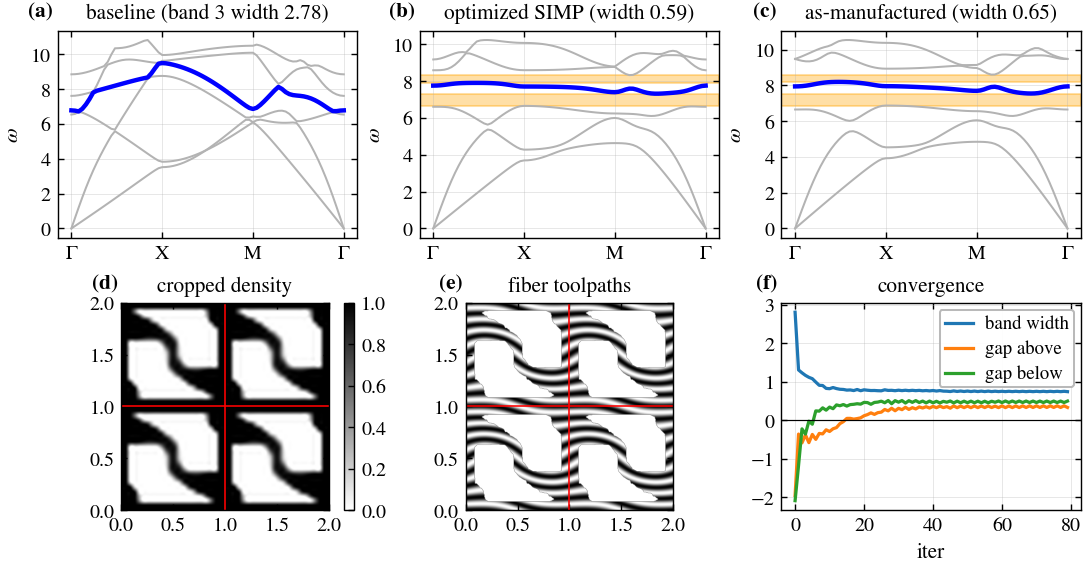
\includegraphics[width=0.99\textwidth]{figs/flatband.png}
\caption{Flat-band $+$ band-gap metamaterial by co-optimized topology and fiber
toolpath, with an as-manufactured validation. Top: band structure
($\Gamma$--X--M--$\Gamma$) of the baseline, the optimized (SIMP) cell, and the
\emph{as-manufactured} cell (cropped density $+$ delineated tows); the target band
$\FBBAND$ (blue) is flattened from $\FBWZ$ to $\FBWO$ and isolated by a gap (orange),
and stays flat ($\FBWV$) with its upper gap ($\FBGUV$) under the manufactured
geometry. Bottom: the crisp (projected) density; the as-manufactured fiber tows
(phase-field wave projection, \S\ref{sec:rbf}, masked to the solid and built from an
exactly cell-periodic phase --- the periodic part by FFT plus an integer number of
tow cycles per period --- so the tows join continuously across all four cell
boundaries), each on a $2\times2$ tiling; and the convergence of the bandwidth and
the two gaps. Design fields: density $z$ \emph{and} orientation $\theta$.}
\label{fig:flatband}
\end{figure}

\subsection{Resolution and toolpath-pitch sweep: what extra design freedom buys}
\label{sec:meta:sweep}
The design freedom in this problem is set by the orientation-support count
$M=k_s^2$, the filter radius $R$, and the tow pitch $d$ of \eqref{eq:scales}. The
analysis mesh $n$ is \emph{not} a design variable --- it is what the physics is
resolved on --- so we hold it fixed at $n=32$, along with the iteration budget,
and vary only the parametrization. This matters: an earlier version of this
experiment refined $n$ together with $(k_s,R,d)$, which forced $N_k$ and the
iteration count \emph{down} as the design freedom went up (the $n^6$ cost of
\eqref{eq:cost}), confounding the two effects beyond recovery.
Table~\ref{tab:sweep} reports the controlled comparison.

% AUTO-GENERATED by examples/flatband_sweep_figure.py -- do not edit.
\begin{table}[h]
\centering
\small
\caption{\textbf{Controlled} design-freedom sweep for the flat-band cell (band $b=3$). The analysis mesh ($n=32$) and the iteration budget (70) are identical for every row, and C1--C3 additionally share one aggregation $\mathbf k$-set ($N_k=22$), so differences between them are attributable to the design parametrization alone: the orientation freedom $M=k_s^2$, the filter radius $R$, and the tow pitch $d$. \textbf{C3d repeats C3 with a denser $\mathbf k$-set} ($N_k=40$) and is the control for $\mathbf k$-sampling. $w_0\!\to\!w_1$ is the target-band width before and after optimization, measured on the common fine $\Gamma$--X--M--$\Gamma$ path; the last three columns are the \emph{as-manufactured} re-simulation (crisp projected density $+$ delineated periodic tows at pitch $d$). Two entries carry the argument of \S\ref{sec:meta:sweep}: C3 is over-parametrized for its $\mathbf k$-set and its true width (0.98) is \emph{worse} than the coarsest design, while C3d --- the same parametrization, sampled adequately --- is the best row on every metric. C1's upper gap goes \emph{negative} once manufactured, its coarse pitch $d=1/6$ being unable to render the design faithfully.}
\label{tab:sweep}
\begin{tabular}{lcccccccccccc}
\toprule
& \multicolumn{4}{c}{design freedom} & \multicolumn{1}{c}{sampling} & \multicolumn{4}{c}{optimized (SIMP, fine path)} & \multicolumn{3}{c}{as-manufactured}\\
\cmidrule(lr){2-5}\cmidrule(lr){6-6}\cmidrule(lr){7-10}\cmidrule(lr){11-13}
run & $k_s$ & $M$ & $R$ & $d$ & $N_k$ & $w_0$ & $w_1$ & $g_\uparrow$ & $g_\downarrow$ & $w^{\rm m}$ & $g^{\rm m}_\uparrow$ & $g^{\rm m}_\downarrow$\\
\midrule
C1 & 4 & 16 & 0.160 & $1/6$ & 22 & 2.87 & 0.66 & +0.16 & +0.58 & 0.84 & -0.14 & +0.36\\
C2 & 6 & 36 & 0.120 & $1/9$ & 22 & 2.52 & 0.56 & +0.22 & +0.45 & 0.65 & +0.21 & +0.52\\
C3 & 8 & 64 & 0.090 & $1/12$ & 22 & 2.06 & 0.98 & +0.13 & +0.12 & 1.02 & +0.08 & +0.11\\
C3d & 8 & 64 & 0.090 & $1/12$ & 40 & 2.06 & 0.55 & +0.53 & +0.67 & 0.55 & +0.59 & +0.57\\
\bottomrule
\end{tabular}
\end{table}


\paragraph{Design freedom helps --- but only if the $\mathbf k$-sampling keeps up.}
Rows C1--C3 share one $\mathbf k$-set ($N_k=22$), so they isolate the
parametrization. Going from $M=16$ to $M=36$ improves the band as expected
($w_1=0.66\to0.56$). Going on to $M=64$ (row C3) does not: the true width
\emph{degrades to} $0.98$, worse than the coarsest design, and both isolating gaps
nearly vanish. Row C3d is the control --- the \emph{same} $M=64$ parametrization,
same mesh, same iterations, with the $\mathbf k$-set enlarged to $N_k=40$ --- and
it is the best row in the table on every metric ($w_1=0.55$,
$g_\uparrow=+0.53$, $g_\downarrow=+0.67$). The finest parametrization was never
the problem; sampling it with $22$ wavevectors was.

The mechanism is \emph{overfitting of the aggregation set}. The KS extrema in
\eqref{eq:flatobj} constrain the band only at the $N_k$ sampled wavevectors. With
$64$ design variables against $22$ samples the design is over-parametrized, and
the optimizer flattens precisely at the samples while the band excurses between
them --- the exact failure the discretization hierarchy \eqref{eq:scales} is meant
to prevent, appearing in the $\mathbf k$-domain rather than the spatial one.

\begin{remark}[A free overfitting diagnostic]
\label{rem:overfit}
The KS bound \eqref{eq:ksbound} makes this detectable at no extra cost. Because
$\widetilde{\max}_\rho$ can only \emph{over}-estimate a maximum (and
$\widetilde{\min}_\rho$ under-estimate a minimum), the aggregated bandwidth is an
upper bound on the true width \emph{over the sampled set}. If the width measured
on a fine path nevertheless comes out \emph{larger} than the aggregate, the band
must be excursing between samples: the design has overfitted the $\mathbf k$-set.
In Table~\ref{tab:sweep} the aggregate widths at the final iterate are $0.79$,
$0.70$, $0.67$ and $0.68$ for C1, C2, C3, C3d, against fine-path widths of
$0.66$, $0.56$, $\mathbf{0.98}$ and $0.55$. Only C3 has fine $>$ aggregate, and
C3 is exactly the row that fails. The test needs no extra optimization --- only one
fine-path evaluation of the converged design.
\end{remark}

\paragraph{Finer tows buy manufacturing fidelity.} The as-manufactured columns
separate the designs again, and along the axis one would expect: the tow pitch.
C1, delineated at the coarse pitch $d=1/6$, does not survive its own toolpath ---
its upper gap goes from $+0.16$ to $\mathbf{-0.14}$, i.e.\ the gap the design was
optimized for \emph{closes} once the fibers are rendered at finite spacing. C2
($d=1/9$) survives with both gaps intact, and C3d ($d=1/12$) is essentially
unchanged by manufacturing ($w_1=0.55\to0.55$, gaps $+0.53/+0.67\to+0.59/+0.57$).
Finer toolpath spacing is therefore not a cosmetic refinement: at $d=1/6$ the
manufactured part does not have the property the design was optimized for.

\begin{figure}[h]
\centering
\IfFileExists{figs/flatband_sweep.png}
  {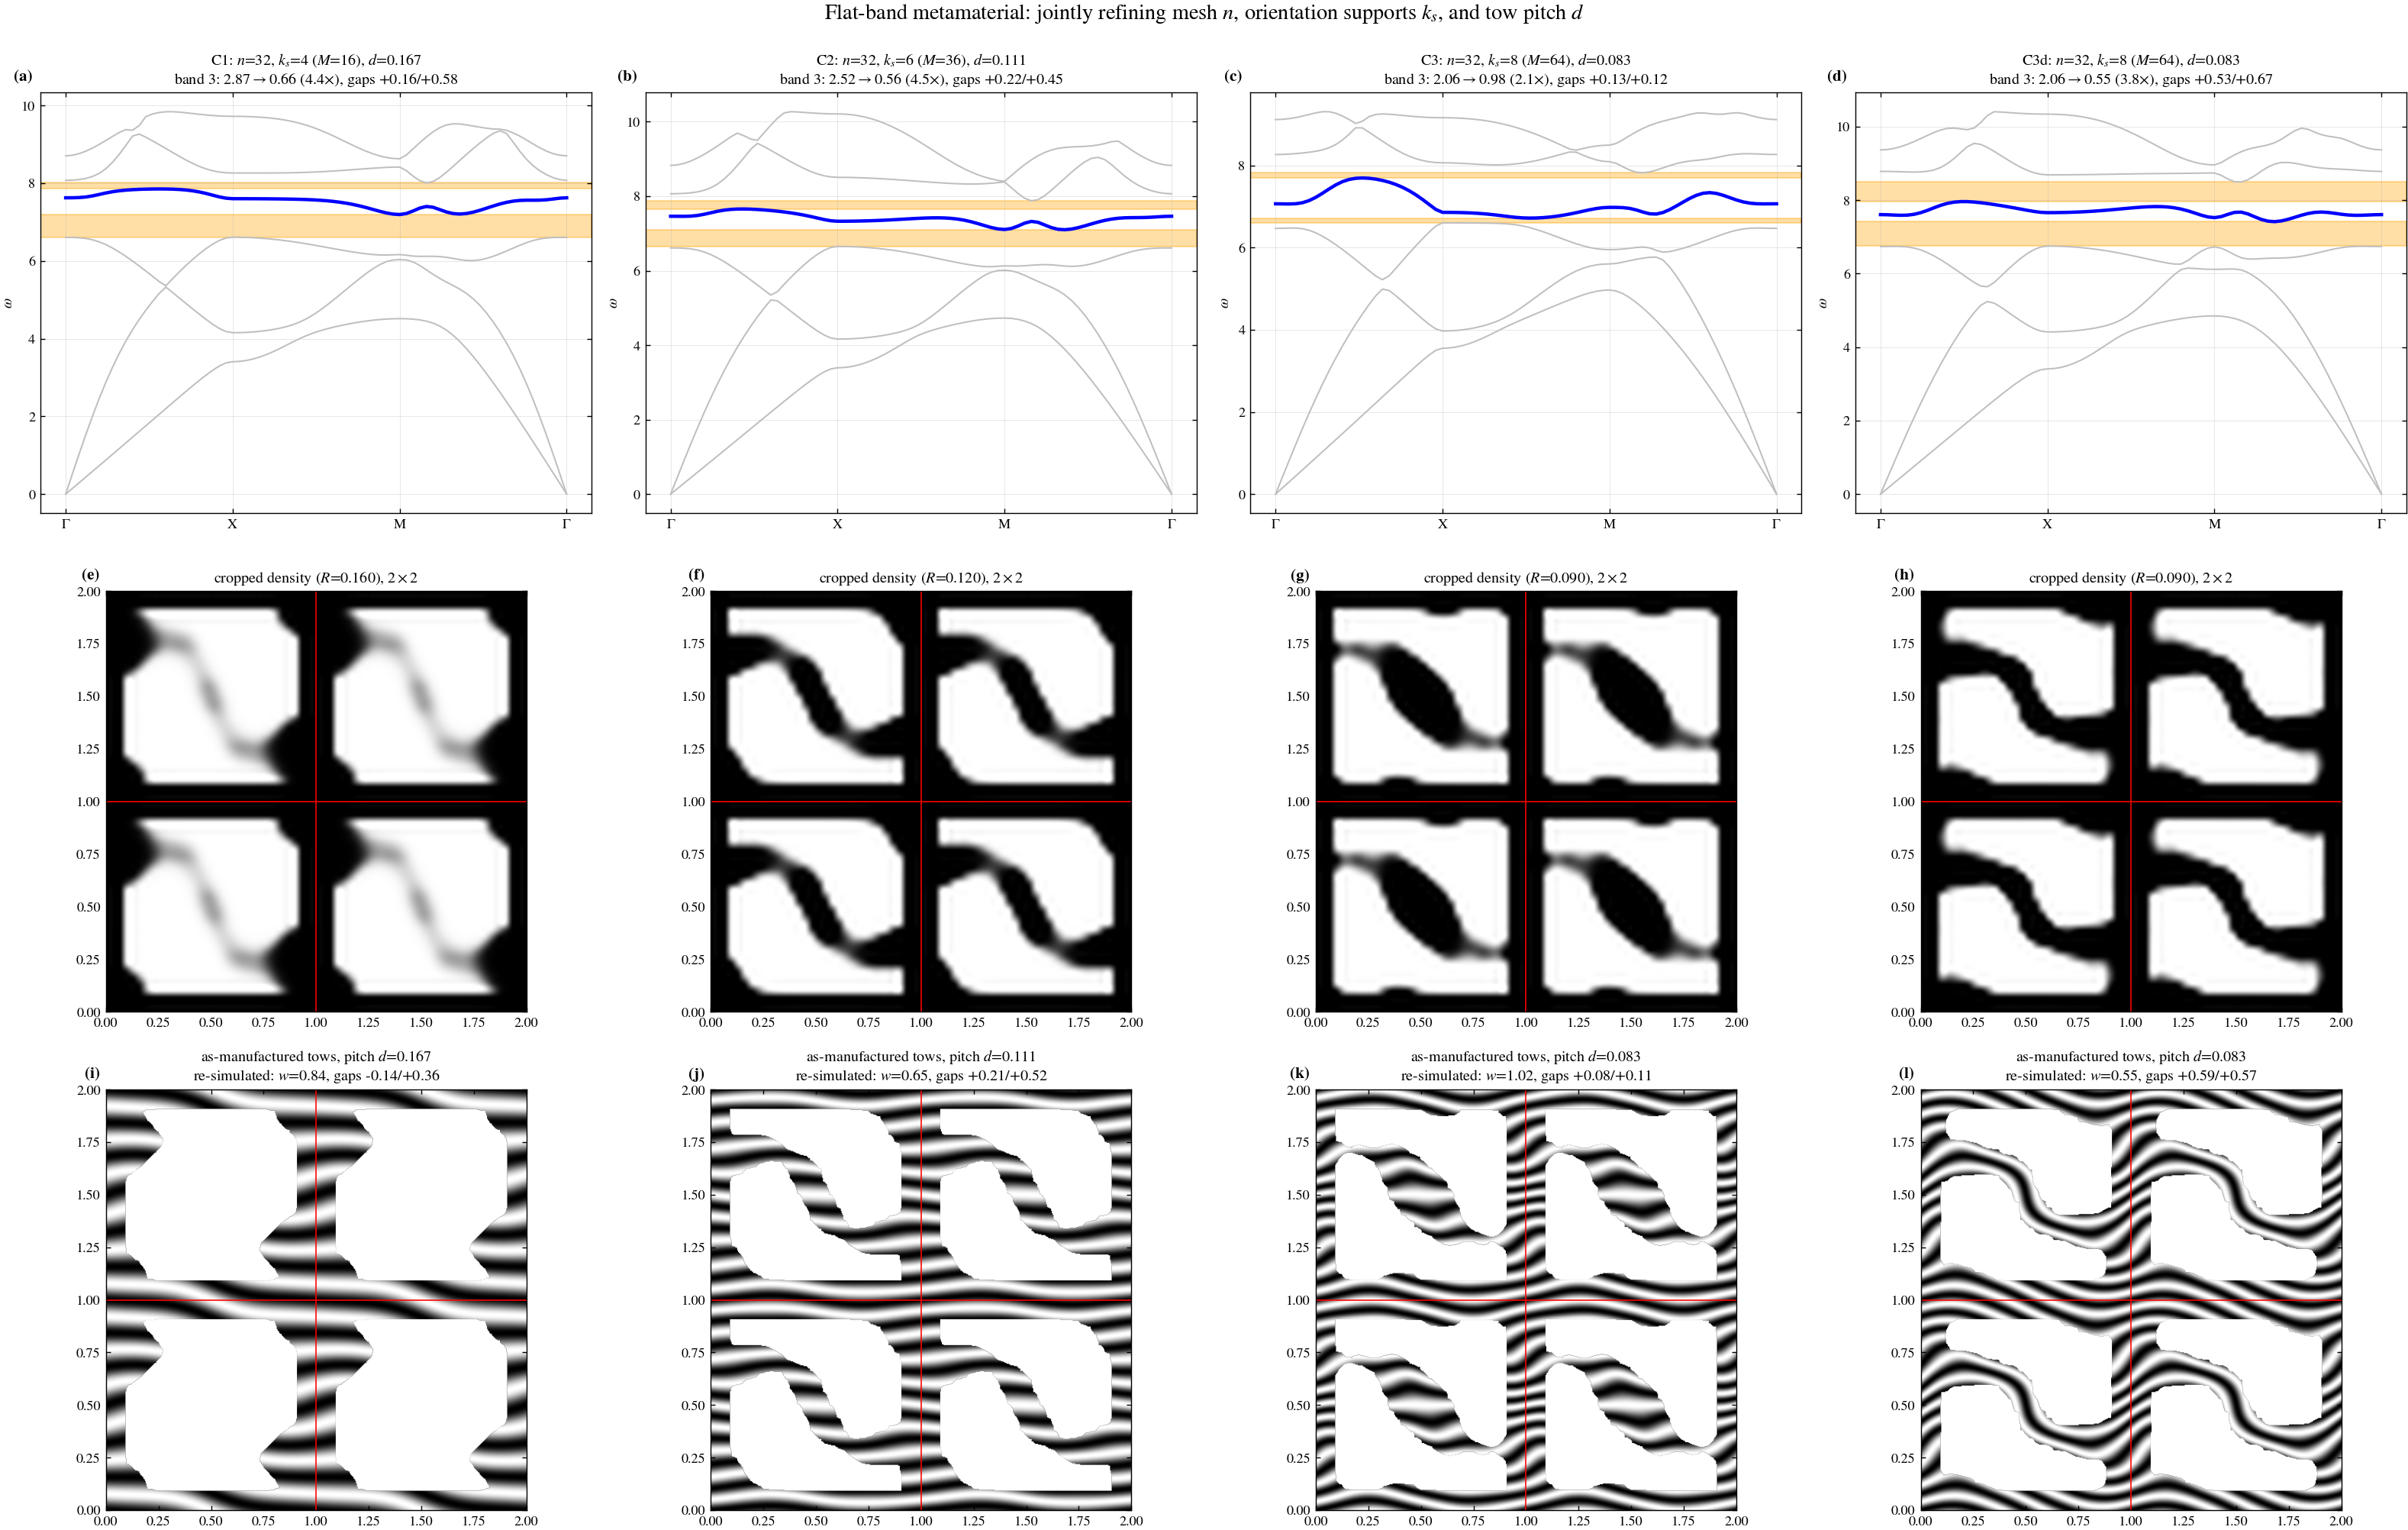
\includegraphics[width=0.99\textwidth]{figs/flatband_sweep.png}}
  {\fbox{\parbox[c][35mm][c]{0.9\textwidth}{\centering\itshape
   figure pending: sweep runs in progress}}}
\caption{Effect of jointly refining the mesh $n$, the orientation-support grid
$k_s$, and the tow pitch $d$. Columns: the three levels of Table~\ref{tab:sweep}.
Top: band structure on the common fine path, with the target band $\FBBAND$ (blue)
and the isolating gaps (orange). Middle: the crisp projected density on a
$2\times2$ tiling --- the finer levels resolve the resonator--frame ligaments that
the coarse cell can only smear. Bottom: the as-manufactured tows at the
corresponding pitch $d$, exactly cell-periodic and masked to the solid.}
\label{fig:sweep}
\end{figure}

\section{Multi-functional design: focusing and stiffness in one fiber layout}
\label{sec:multifunc}
A structural panel often has to do two jobs at once: carry a mechanical load, and
manage an elastic wave. This section poses both on a single finite part and asks
whether one fiber layout can serve both --- a genuine multi-functional co-design,
on a finite domain, with \emph{no band gap} anywhere.

\paragraph{Why not the periodic band-gap route.}
The natural first attempt is a periodic cell co-designed for homogenized
stiffness and a complete phononic band gap. We pursued that and report its
failure plainly, because it is instructive. The complete gap was aggregated over
a discrete $\mathbf k$-sample during optimization; the optimizer drove the gap
open \emph{at the sampled points} while the bands crossed \emph{between} them, so
the ``gaps'' were artifacts of sparse $\mathbf k$-sampling. Re-evaluating the
optimized cells on a dense $11\times11$ Brillouin-zone grid, the reported gaps of
$+0.21$, $+0.39$ and $+0.55$ became $-0.20$, $-0.09$ and $+0.08$ --- essentially
closed --- and straightening the fibers \emph{widened} the true gap in every
case, so the orientation was gaming the coarse metric rather than opening a gap.
A band-gap claim is only as good as its $\mathbf k$-convergence, and this one did
not survive it. We therefore move the multi-functional demonstration to a finite
domain, where the objectives are integrals over the part rather than extrema over
a Brillouin zone and no such sampling gap exists.

\subsection{Two objectives on one solid plate}
On the $4\times3$ solid orthotropic plate of \S\ref{sec:results}, driven at
$\omega=40$ by the left-edge plane wave, the fiber orientation $\theta(\vx)$ is
scored on
\begin{itemize}\itemsep0pt
  \item \textbf{dynamic:} the focus gain $G=E_{\rm foc}(\theta)/E_{\rm foc}(0)$,
        the focus-region energy relative to straight fibers (the lens objective
        of \S\ref{sec:results}, adjoint FD-verified to $\FLFDFOC$ digits);
  \item \textbf{static:} the cantilever compliance $c=\mathbf{F}_s\T\vu_s$ with
        $\mathbf{K}(\theta)\vu_s=\mathbf{F}_s$ --- the left edge clamped, a transverse load on
        the right edge. Compliance is self-adjoint, $\partial c/\partial\theta=
        -\vu_s\T(\partial\mathbf{K}/\partial\theta)\vu_s$, FD-verified to $\FLFDC$.
\end{itemize}
Both are functions of the same $\theta$ on the same plate. The tension is real:
the converging-lens layout that bends the wave toward the target is not the
load-aligned layout that resists bending.

\subsection{Result: one layout, both functions}
Three designs from an identical straight-fiber start make the point. The
\emph{focus-only} lens reaches a focus gain of
$\FLFOCONLY\times$ but drops the panel stiffness to $\FLFOSTIFF\times$ that of
straight fibers --- steering the wave costs $\FLFOCOST\%$ of the structural
stiffness. Constraining the compliance to the straight-fiber level and
maximizing focus (augmented Lagrangian on the single compliance constraint,
 as in \S\ref{sec:curl}) gives the
\emph{co-design}: a focus gain of $\FLCOFOC\times$ at $\FLCOSTIFF\times$ the
straight-fiber stiffness --- essentially all of the stiffness \emph{and} a large
fraction of the focusing, from one fiber field.

Sweeping the compliance limit traces the focus--stiffness front:
focus gain rises from $\FLCOFOC\times$
at full stiffness, through $\FLKNEE\times$ at a $20\%$ compliance allowance, to
the focus-only endpoint, saturating once the stiffness constraint is loose enough
to stop binding. The designer reads an operating point off this curve rather than
choosing between the two functions. Unlike the periodic band-gap result, every
point here is an integral over the finite part and carries no $\mathbf k$-sampling
caveat.

\section{Wave shielding on a solid CFRP plate with drilled holes}
\label{sec:codesign}
The multi-functional result of \S\ref{sec:multifunc} designs the fiber orientation
alone, on a solid homogeneous plate. A real composite panel adds one feature the
orientation-only picture omits: \emph{prescribed through-holes} --- bolt holes,
fastener passages, access cut-outs --- whose rims are traction-free boundaries the
wave scatters from. Here we turn that feature into an asset. Exactly as the elastic
cloak (\S\ref{sec:cloak}) wraps the fiber toolpath around a real hole to control its
scattered field, we design the toolpath of a \emph{holed} panel to \emph{shield}
sensitive regions: harmonic vibration enters at \emph{both} bottom corners --- two
independent source load cases --- and the fiber layout must divert it away from
\emph{both} of the opposite top corners, across a \emph{band} of frequencies, while
the holes cut weight and the fiber alignment keeps the panel stiff.

Insisting on \emph{real} holes here --- cut from the geometry, with no material
inside --- rather than soft-density voids is decisive for a wave objective. A wave
localizes in the slow, compliant phase, so a soft-density void \emph{attracts} the
field: any weight saved by softening material reappears as wave energy sitting in
what looks like a void, and a mass objective and a wave objective end up fighting
over the same cells. A traction-free hole does the opposite --- the wave reflects off
its rim and cannot enter --- so the shielded field lives entirely in solid material,
there is provably zero wave energy in any void, and mass reduction and wave control
stop competing. This is the cloak's mechanism (orientation control around real holes),
aimed at a protected region instead of at invisibility.

\subsection{A conforming vector element: the missing discretization}
\label{sec:codesign:cst}
Every in-plane (vector) result in this paper so far lives on a structured quad grid;
every result on a hole-conforming \texttt{gmsh} triangulation is scalar antiplane
(\S\ref{sec:spaces}). This problem needs \emph{both at once} --- vector elasticity on
a mesh that conforms to holes --- so we add the element that was missing: a
constant-strain-triangle (CST) plane-stress element carrying the same rotated
orthotropic fiber stiffness $\mathbf D_f(\theta)$ as the quad elements. It reuses,
unchanged, the exact five-term Fourier decomposition of Appendix~\ref{app:fourier}:
with $\mathbf B$ the $3\times6$ CST strain-displacement matrix and $A$ the triangle
area,
\begin{equation}
  \mathbf k_f(\theta)=\sum_{s=0}^{4} c_s(\theta)\,\underbrace{A\,\mathbf B\T
    \mathbf C_s\,\mathbf B}_{\text{5 fixed }6\times6\text{ matrices}},\qquad
  \mathbf c(\theta)=\bigl[1,\ \cos2\theta,\ \sin2\theta,\ \cos4\theta,\ \sin4\theta\bigr],
  \label{eq:cstfourier}
\end{equation}
so element rotation is five precomputed matrices weighted by trigonometric scalars,
and $\partial\mathbf k_f/\partial\theta$ costs only the derivative of
$\mathbf c(\theta)$. The mesh is built by cutting the disks from the rectangle in the
OCC kernel, giving \emph{exactly} circular, traction-free rims (a natural boundary
condition), graded finer toward each rim --- never a soft-density staircase, for the
scattering reasons argued in \S\ref{sec:valley:mesh}. The Fourier fit is exact to
$8.5\times10^{-16}$, and both design adjoints (the dynamic protected-energy and the
static compliance, each w.r.t.\ $\theta$) pass the finite-difference check to
$\lesssim10^{-6}$.

\subsection{Result: a shielded region, entirely in solid material, at lower mass}
\label{sec:codesign:result}
On a $7\times4$ panel carrying five drilled through-holes (radii $0.48$--$0.60$),
meshed conformally, harmonic vibration enters at \emph{both} bottom corners --- two
independent source load cases --- and we ask that it stay out of \emph{both} top
corners across a band of frequencies $\omega\in\{9,11,13\}$
(Figure~\ref{fig:codesign}, Table~\ref{tab:codesign}). With straight fibers,
$7$--$12\%$ of the interior energy reaches the protected corners at each frequency.
Minimizing the band-averaged protected energy --- summed over both sources, with one
LU factorization per frequency serving every source load case --- over the fiber
orientation, with a printable-curvature penalty and a compliance term and only the
orientation as a variable, diverts the wave: the protected fraction falls to
$2$--$3\%$, a $3$--$5\times$ reduction \emph{at every frequency}, with both corners
dark across the whole band while the field stays brightest at the two sources. Every
bright region is solid, and every hole shows exactly zero energy inside, because the
wave cannot enter a real void. The same layout is $24\%$ stiffer than straight fiber
and, through the five holes, $15\%$ lighter than the full plate, at a maximum fiber
curvature $|\zeta|_{\max}=1.1$ --- inside the $1/R$ bound of the smallest hole, so the
tows are printable. The orientation gradient is finite-difference verified to
$\lesssim10^{-6}$ and, by the isotropy-annihilation identity (Remark~\ref{rem:iso}),
driven purely by the fiber anisotropy: setting $\mathbf Q_f$ isotropic sends every
$\partial E/\partial\theta$ to $O(10^{-16})$.

\begin{table}[!htbp]
\centering\small
\caption{Broadband, two-source, multi-target fiber-orientation wave shield on the
holed CFRP panel: the share of interior energy reaching the union of the two protected
top corners (summed over the two bottom-corner source load cases), straight fibers
versus the optimized toolpath, at each frequency. The single optimized layout is
$0.76\times$ the straight-fiber cantilever compliance ($24\%$ stiffer) at a maximum
fiber curvature $|\zeta|_{\max}=1.1$ (printable). Both designs carry the same five
drilled holes, so both are $0.85\times$ the solid-plate mass, and by construction
neither has any wave energy in a void.}
\label{tab:codesign}
\begin{tabular}{cccc}
\toprule
frequency $\omega$ & straight fraction & optimized fraction & quieter\\
\midrule
$9$  & $0.070$ & $\mathbf{0.022}$ & $\mathbf{3\times}$\\
$11$ & $0.119$ & $\mathbf{0.026}$ & $\mathbf{5\times}$\\
$13$ & $0.117$ & $\mathbf{0.029}$ & $\mathbf{4\times}$\\
\bottomrule
\end{tabular}
\end{table}

\begin{figure}[!htbp]
\centering
\IfFileExists{figs/cfrp_wave_shield.png}
  {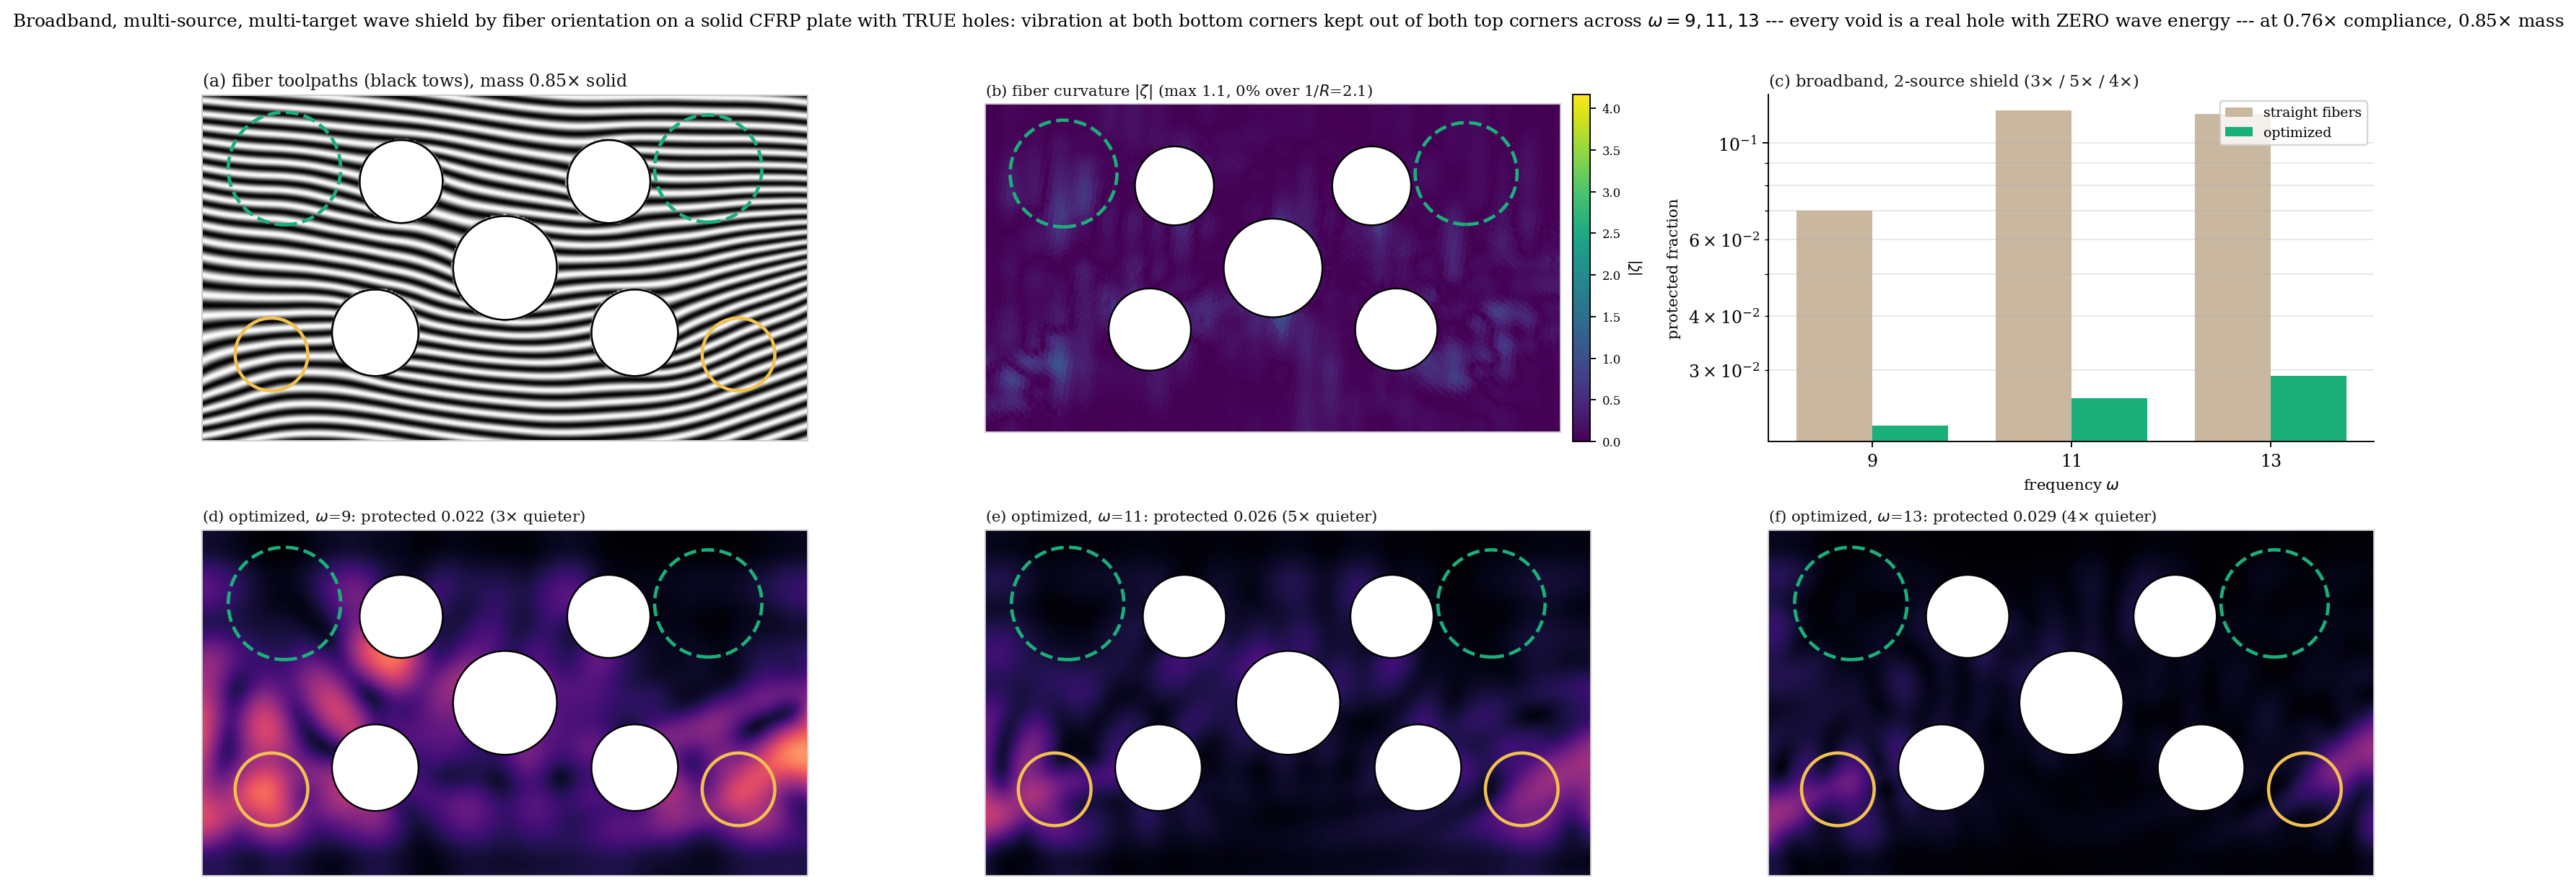
\includegraphics[width=0.99\textwidth]{figs/cfrp_wave_shield.png}}
  {\fbox{\parbox[c][35mm][c]{0.9\textwidth}{\centering\itshape
   figure pending: run in progress}}}
\caption{Broadband, two-source, multi-target fiber-orientation wave shield on a solid
CFRP plate with five drilled through-holes. Vibration enters at \emph{both} bottom
corners (yellow) and must be kept out of \emph{both} top-corner regions (green dashed)
across $\omega\in\{9,11,13\}$. (a) The optimized fiber toolpath, drawn as tows on the
solid with the holes cut out; $0.85\times$ the solid-plate mass. (b) The fiber
curvature $|\zeta|$ (max $1.1$, everywhere inside the $1/R$ print limit). (c) The
protected-corner energy fraction at each frequency, straight fibers versus optimized:
the shield reduces it $3$--$5\times$ across the band. (d--f) The combined field over
the two sources at $\omega=9,11,13$: both corners stay dark at every frequency, the
field is brightest at the sources, and every hole is a real void with exactly zero
wave energy inside --- the shielded field is entirely in solid material.}
\label{fig:codesign}
\end{figure}

This is the cloak's anisotropy lever (\S\ref{sec:cloak}) aimed at a protected region
rather than at invisibility, and it settles the tension that a soft-void topology
cannot: because the removed material is real holes, not compliant voids, the wave has
nowhere soft to collect, so the panel is lighter \emph{and} the shielded field never
leaves the solid. Nothing in the objective is periodic and every quantity is an
integral over a finite, buildable part.

\section{A stiffer, stronger bracket with a higher fundamental: topology and toolpath
for a modal objective}
\label{sec:bracket}
The shield of \S\ref{sec:codesign} designs a toolpath on a fixed hole pattern. Our
last finite-part example designs \emph{both} the topology and the toolpath, and
targets a \emph{modal} objective, using the eigenvalue sensitivity that drives the
metamaterial of \S\ref{sec:meta} --- here on a clamped finite part rather than a Bloch
cell. The part is a mounting bracket: bolted at two holes on the clamped root and
carrying a service load on the rim of a third through-hole at the tip, it should have
the highest possible first natural frequency $\omega_1$ --- to keep the fundamental
resonance clear of the operating excitation --- at a \emph{fixed mass}. Maximizing a
single eigenvalue in isolation is a trap: because a Rayleigh quotient rewards any mass
placed where it raises stiffness faster than inertia, the optimizer readily grows
\emph{neutral outriggers} --- stubby cantilevers near the root that nudge $\omega_1$ up
by a hair but carry no service load, so the ``bracket'' sprouts dead appendages
(removing them changes $\omega_1$ by under half a percent but they persist in every
volume-constrained run, regrowing even when their region is forbidden). We therefore
co-design against \emph{three} objectives at once, all at fixed mass: maximize
$\omega_1$; minimize the static compliance, so every member is load-bearing rather than
a frequency outrigger; and minimize the peak stress, so the load path is thick and
uniformly stressed rather than a set of thin overloaded ligaments. It is a single solid
anisotropic material --- no fiber/matrix blend, only fiber and true void (a $1\%$ Ersatz
keeps the operators non-singular) --- so ``mass'' here counts only real material, the
compliance and the p-norm von Mises peak stress (Appendix~\ref{app:stresssens}) are both
taken under the tip load, and each carries its own adjoint.

\paragraph{The counterintuitive lever.} It is tempting to read ``higher $\omega_1$''
as simply ``stiffer.'' But $\omega_1^2$ is a Rayleigh quotient
$\bm\phi\T\mathbf K\bm\phi/\bm\phi\T\mathbf M\bm\phi$, and its density sensitivity
\eqref{eq:eigsens_z} carries two terms of opposite sign: a positive stiffness term
that wants material where the mode strains, and a \emph{negative} mass term,
$-\lambda_1(\rho_f-\rho_m)\,\bm\phi_e\T\mathbf m_0\bm\phi_e$, that wants material
\emph{removed} where the mode has kinetic energy --- at its antinodes. At a fixed mass
budget the optimizer plays these against each other: it draws material toward the
strained root and \emph{scoops it out of the antinode at the tip}, so the fundamental
rises far more than the change in total stiffness alone would suggest. The compliance
and peak-stress objectives keep that redistribution physical and honest: compliance
forces the redistributed material onto genuine load paths rather than the neutral root
outriggers a bare eigenvalue objective would grow, and the peak-stress term spreads
those paths into thick, uniformly stressed members rather than thin overloaded
ligaments.

\paragraph{The design we build.} We solve the bracket on a fine $3.5\times2$ mesh
(${\sim}68\rm k$ elements), enforcing mirror symmetry about the mid-height axis,
clamp-connectivity (only material grounded to the support survives, so there are no
floating islands), and thin passive-solid collars backing every hole; every ratio is
against an \emph{equal-mass} uniform-density plate. The manufacturable result is the
clean, fully load-bearing A-frame of Figure~\ref{fig:bracket}: a top chord in tension and
a bottom chord in compression sweeping from the clamped root to the loaded tip ring, the
fiber tows wrapping every hole and following each chord. The tension/compression map
(Figure~\ref{fig:bracket}b) shows \emph{every member carries load} --- there are no dead
appendages. It is $7.3\times$ stiffer than the equal-mass plate, holds the peak stress to
$0.15\times$, and raises the fundamental to $2.83\times$; that rise is \emph{proportionate}
($\omega_1^2$ tracks the stiffness gain) --- the honest reading of ``higher $\omega_1$
means stiffer.'' The design is binary ($M_{\rm nd}=0.02$) and printable: an adaptive
curvature penalty drives $|\zeta|_{\max}$ right up to the AFP limit $1/R$ --- the tows use
the \emph{full} manufacturability budget to follow the load --- and no further.

\paragraph{The frequency lever, and why we do not build it.} The modal objective can push
the fundamental much higher, but not for free. Sweeping the modal weight $w_\omega$ from
$0$ to $1$ traces the stiffness--frequency evolution of Figure~\ref{fig:pareto}: the
pure-stiffness A-frame sits \emph{on} the proportionate line $\omega_1^2\!\propto\!$~
stiffness, and the first touch of frequency weight lifts the design far above it into the
\emph{disproportionate} region --- $\omega_1$ climbs toward $3.8$--$4\times$, so
$\omega_1^2$ rises ${\sim}14$--$16\times$ against only a ${\sim}5\times$ stiffness gain,
the extra factor being mass scooped off the mode's tip antinode via the
$-\lambda_1\,\partial\mathbf M/\partial z$ term (against a \emph{fully solid} plate the
frequency-weighted design more than doubles $\omega_1$ at $0.42\times$ its mass). But that
extra frequency is bought with lightly-loaded \emph{modal} material: the frequency-weighted
designs grow an inner arrow and stubby outriggers that a tension/compression check shows
carry almost no service load --- they reshape the mode, not the load path. Trimming them
costs under $2\%$ of $\omega_1$ and returns the A-frame. So the lever is real and
physically interesting, but the load-bearing, manufacturable part is the clean A-frame ---
the sweep is how we know exactly what the lever would cost to build.

\paragraph{Mode separation by anisotropy.} The same eigenvalue machinery does something
the load path cannot: play $\omega_1$ against $\omega_2$. Maximizing $\omega_1$ \emph{while
minimizing} $\omega_2$ --- with a second-mode eigenvalue adjoint (Appendix~\ref{app:modalsens})
alongside the first --- drives the two lowest natural frequencies \emph{together}: the gap
$\omega_2/\omega_1$ collapses from ${\sim}4$ toward ${\sim}\BRTWOGAP$ as the mode-2 weight
$w_2$ is raised (Figure~\ref{fig:mode2}), tuning the bracket toward a near-degenerate
fundamental pair. It is a purely anisotropic effect --- the fiber field stiffens the first
mode's strain field while softening the second's, which an isotropic redesign at fixed
mass cannot do as sharply --- and a stringent test of the sensitivities near an eigenvalue
crossing.

\paragraph{Designed anisotropy is doing the work.} The fiber orientation is a full design
field, not a fixed layup. On the frozen A-frame topology the optimized tows are $44\%$
stiffer than the best straight, single-angle laminate: the anisotropy is designed, not
incidental. The tows run along the chords and wrap every hole (Figure~\ref{fig:bracket}a),
putting the $E_{f1}=131$~GPa axis on the load to within ${\sim}6^\circ$ of the principal
stress on every loaded member. The rotated stiffness $D_f(\theta)=\mathbf T\mathbf Q_f
\mathbf T\T$ reproduces the analytical off-axis modulus $E_x(\theta)$ --- from $131$~GPa
along the fiber to $9$~GPa across --- to machine precision, and the finer the fiber field
is resolved the harder the tows follow the load: a coarse support grid flattens them
artificially, leaving ${\sim}30\%$ of the anisotropy on the table. Tellingly, the
\emph{modal} objective reaches for anisotropy hardest --- left unpenalized its tows would
curl to $|\zeta|\!\approx\!14$ versus ${\approx}2$ for the compliance design, so the
printability penalty binds on the frequency design first. All sensitivities --- the two
eigenvalue sensitivities for $\omega_1$ \emph{and} $\omega_2$ (density and orientation,
\S\ref{app:modalsens}), the compliance adjoint, and the p-norm stress adjoint
(\S\ref{app:stresssens}) --- are finite-difference verified to $\lesssim10^{-6}$, and
every orientation gradient isotropy-annihilates.

\begin{figure}[!htbp]
\centering
\IfFileExists{figs/cfrp_bracket_hero.png}
  {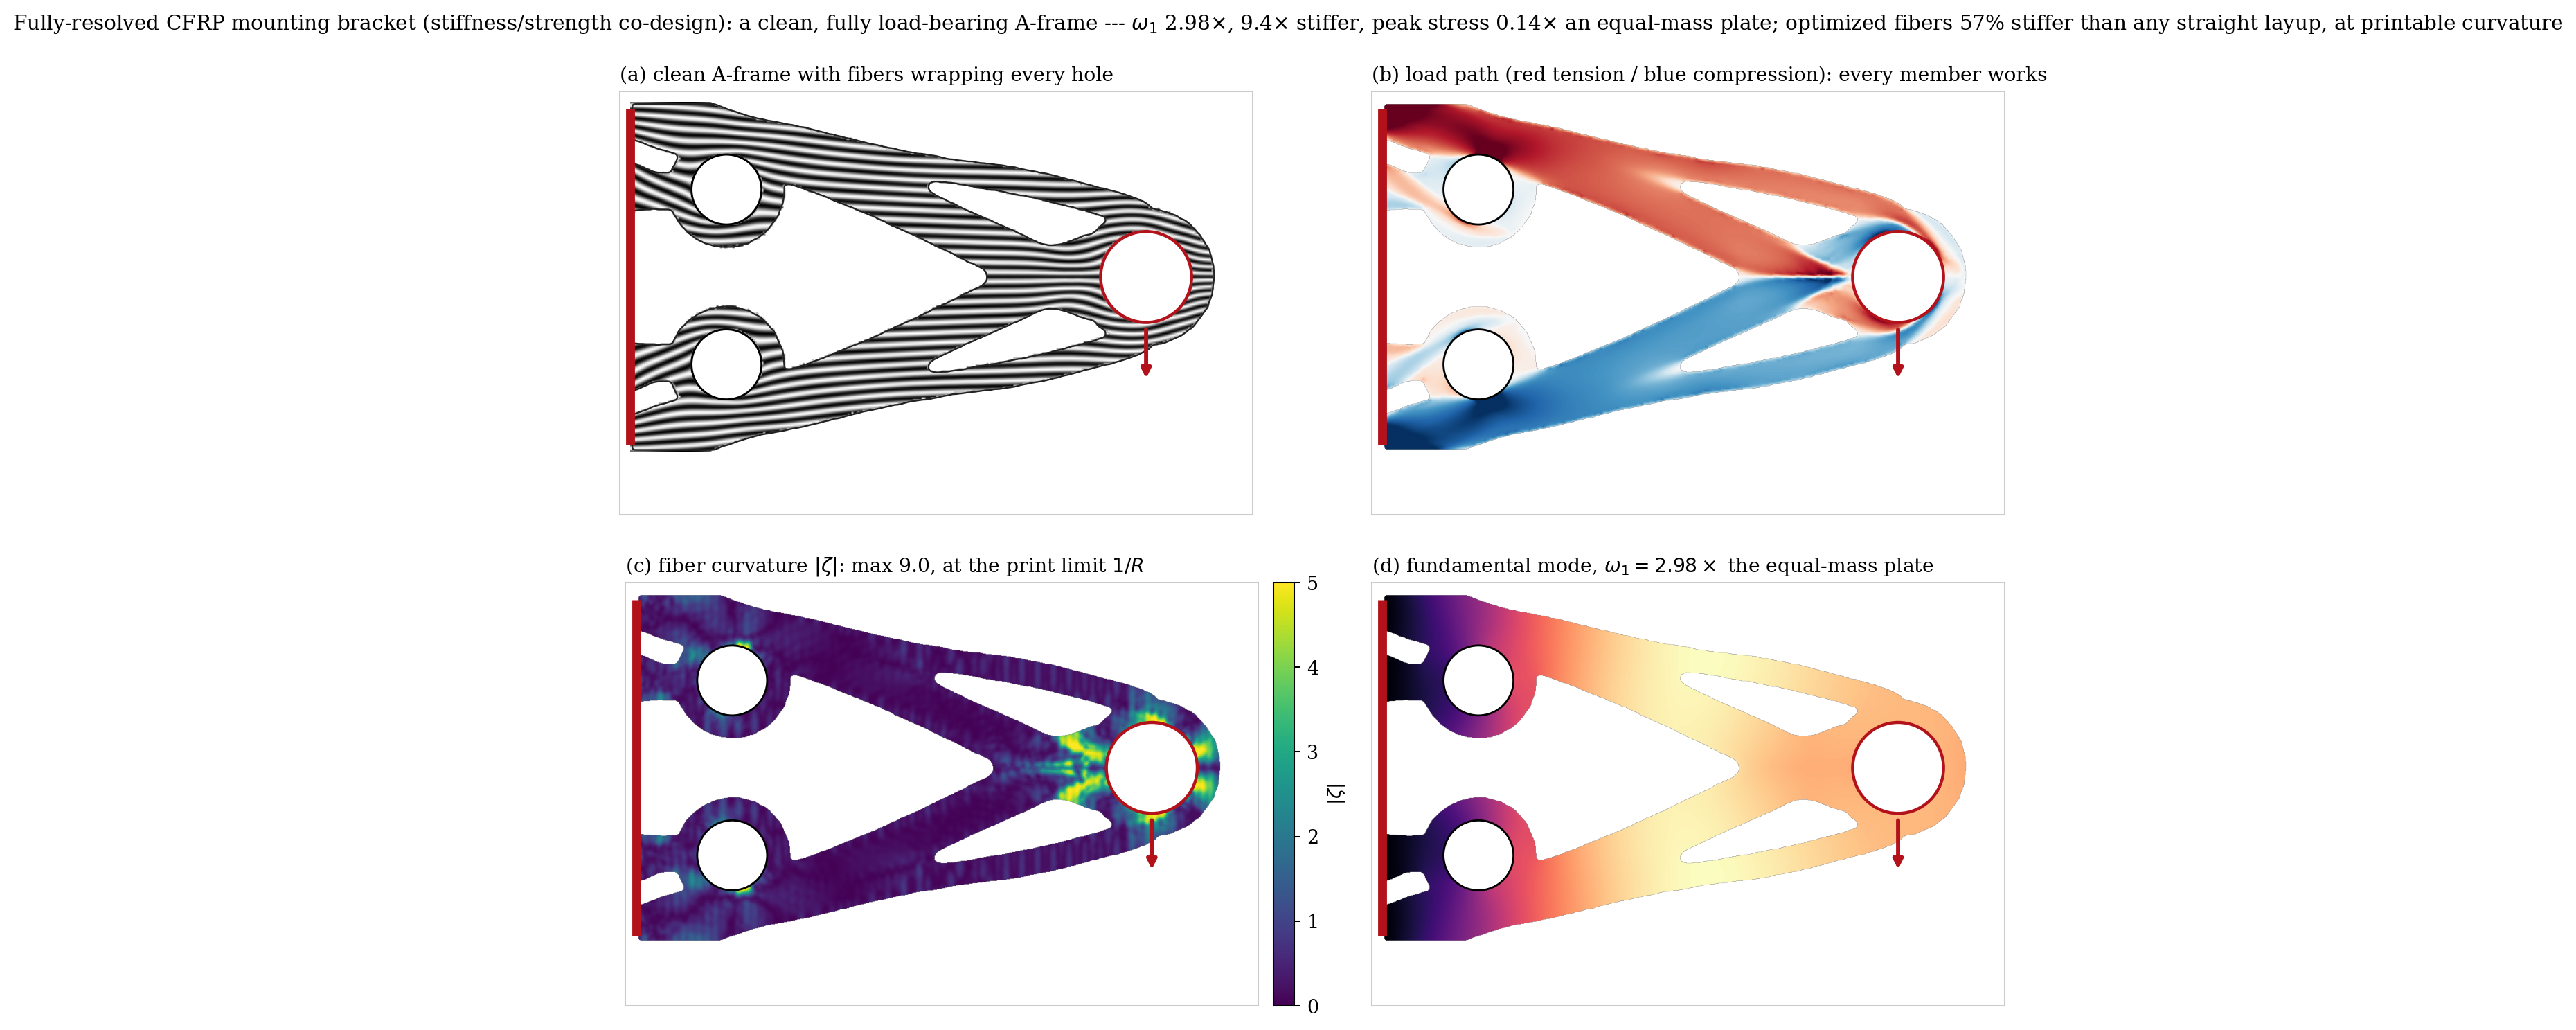
\includegraphics[width=0.98\textwidth]{figs/cfrp_bracket_hero.png}}
  {\fbox{\parbox[c][32mm][c]{0.9\textwidth}{\centering\itshape
   figure pending: run in progress}}}
\caption{The fully-resolved CFRP mounting bracket (stiffness/compliance/stress co-design,
${\sim}68\rm k$ elements): a clean, fully load-bearing A-frame at equal mass. Bolted at
two root holes (clamp edge, red), loaded on the tip-hole rim (red); thin passive-solid
collars back every hole. (a) Topology with the continuous fiber tows, which \emph{wrap
every hole} and follow each chord. (b) The load path (red tension, blue compression): a
top tension chord and a bottom compression chord --- \emph{every} member carries load,
with no dead appendages. (c) Fiber curvature $|\zeta|$, driven right to the print limit
$1/R$ so the tows exploit the full manufacturability budget. (d) The fundamental mode,
$\omega_1=2.83\times$ the equal-mass plate. The design is $7.3\times$ stiffer and holds
the peak stress to $0.15\times$; its optimized fibers are $44\%$ stiffer than any straight
layup.}
\label{fig:bracket}
\end{figure}

\begin{figure}[!htbp]
\centering
\IfFileExists{figs/cfrp_bracket_pareto.png}
  {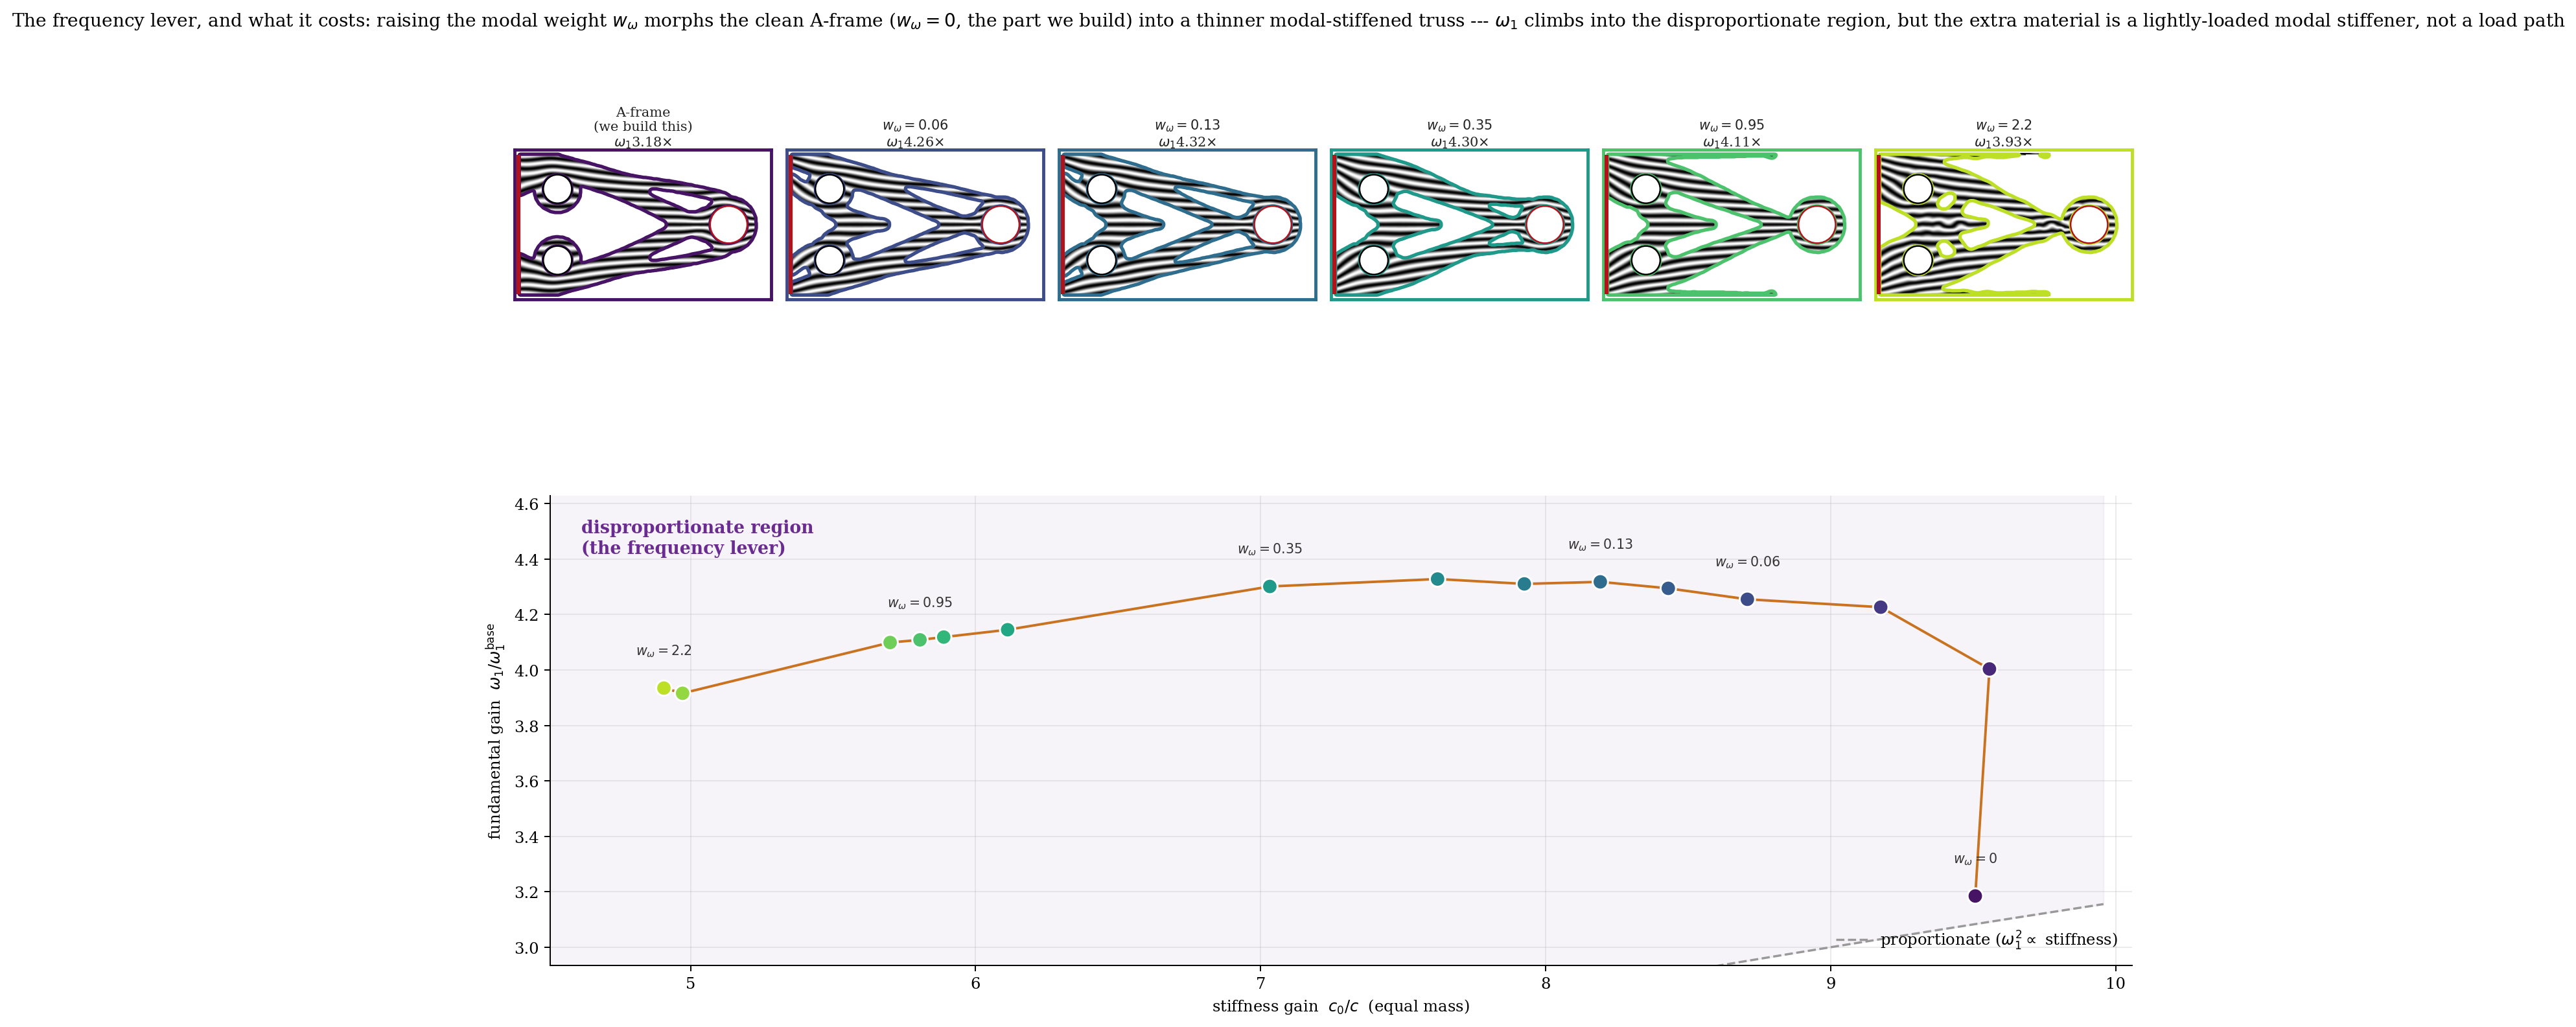
\includegraphics[width=0.99\textwidth]{figs/cfrp_bracket_pareto.png}}
  {\fbox{\parbox[c][32mm][c]{0.9\textwidth}{\centering\itshape
   figure pending: run in progress}}}
\caption{The frequency lever, and what it costs. Sweeping the modal weight $w_\omega$ from
$0$ (the manufacturable A-frame of Figure~\ref{fig:bracket}) to $1$ (frequency-weighted)
traces the stiffness--frequency evolution at equal mass. \emph{Top:} the part morphs from
the clean A-frame into a thinner truss with an inner arrow and outriggers as $w_\omega$
rises. \emph{Bottom:} the pure-stiffness design lands on the proportionate line
$\omega_1\!=\!\sqrt{\text{stiffness}}$ (dashed); any frequency weight lifts it into the
\emph{disproportionate} region above --- $\omega_1$ reaches $3.8$--$4\times$
($\omega_1^2\!\sim\!14$--$16\times$ the stiffness gain). The catch is that the extra
material is a lightly-loaded modal stiffener, not a load path, so the design we build is
the $w_\omega{=}0$ end.}
\label{fig:pareto}
\end{figure}

\begin{figure}[!htbp]
\centering
\IfFileExists{figs/cfrp_bracket_mode2.png}
  {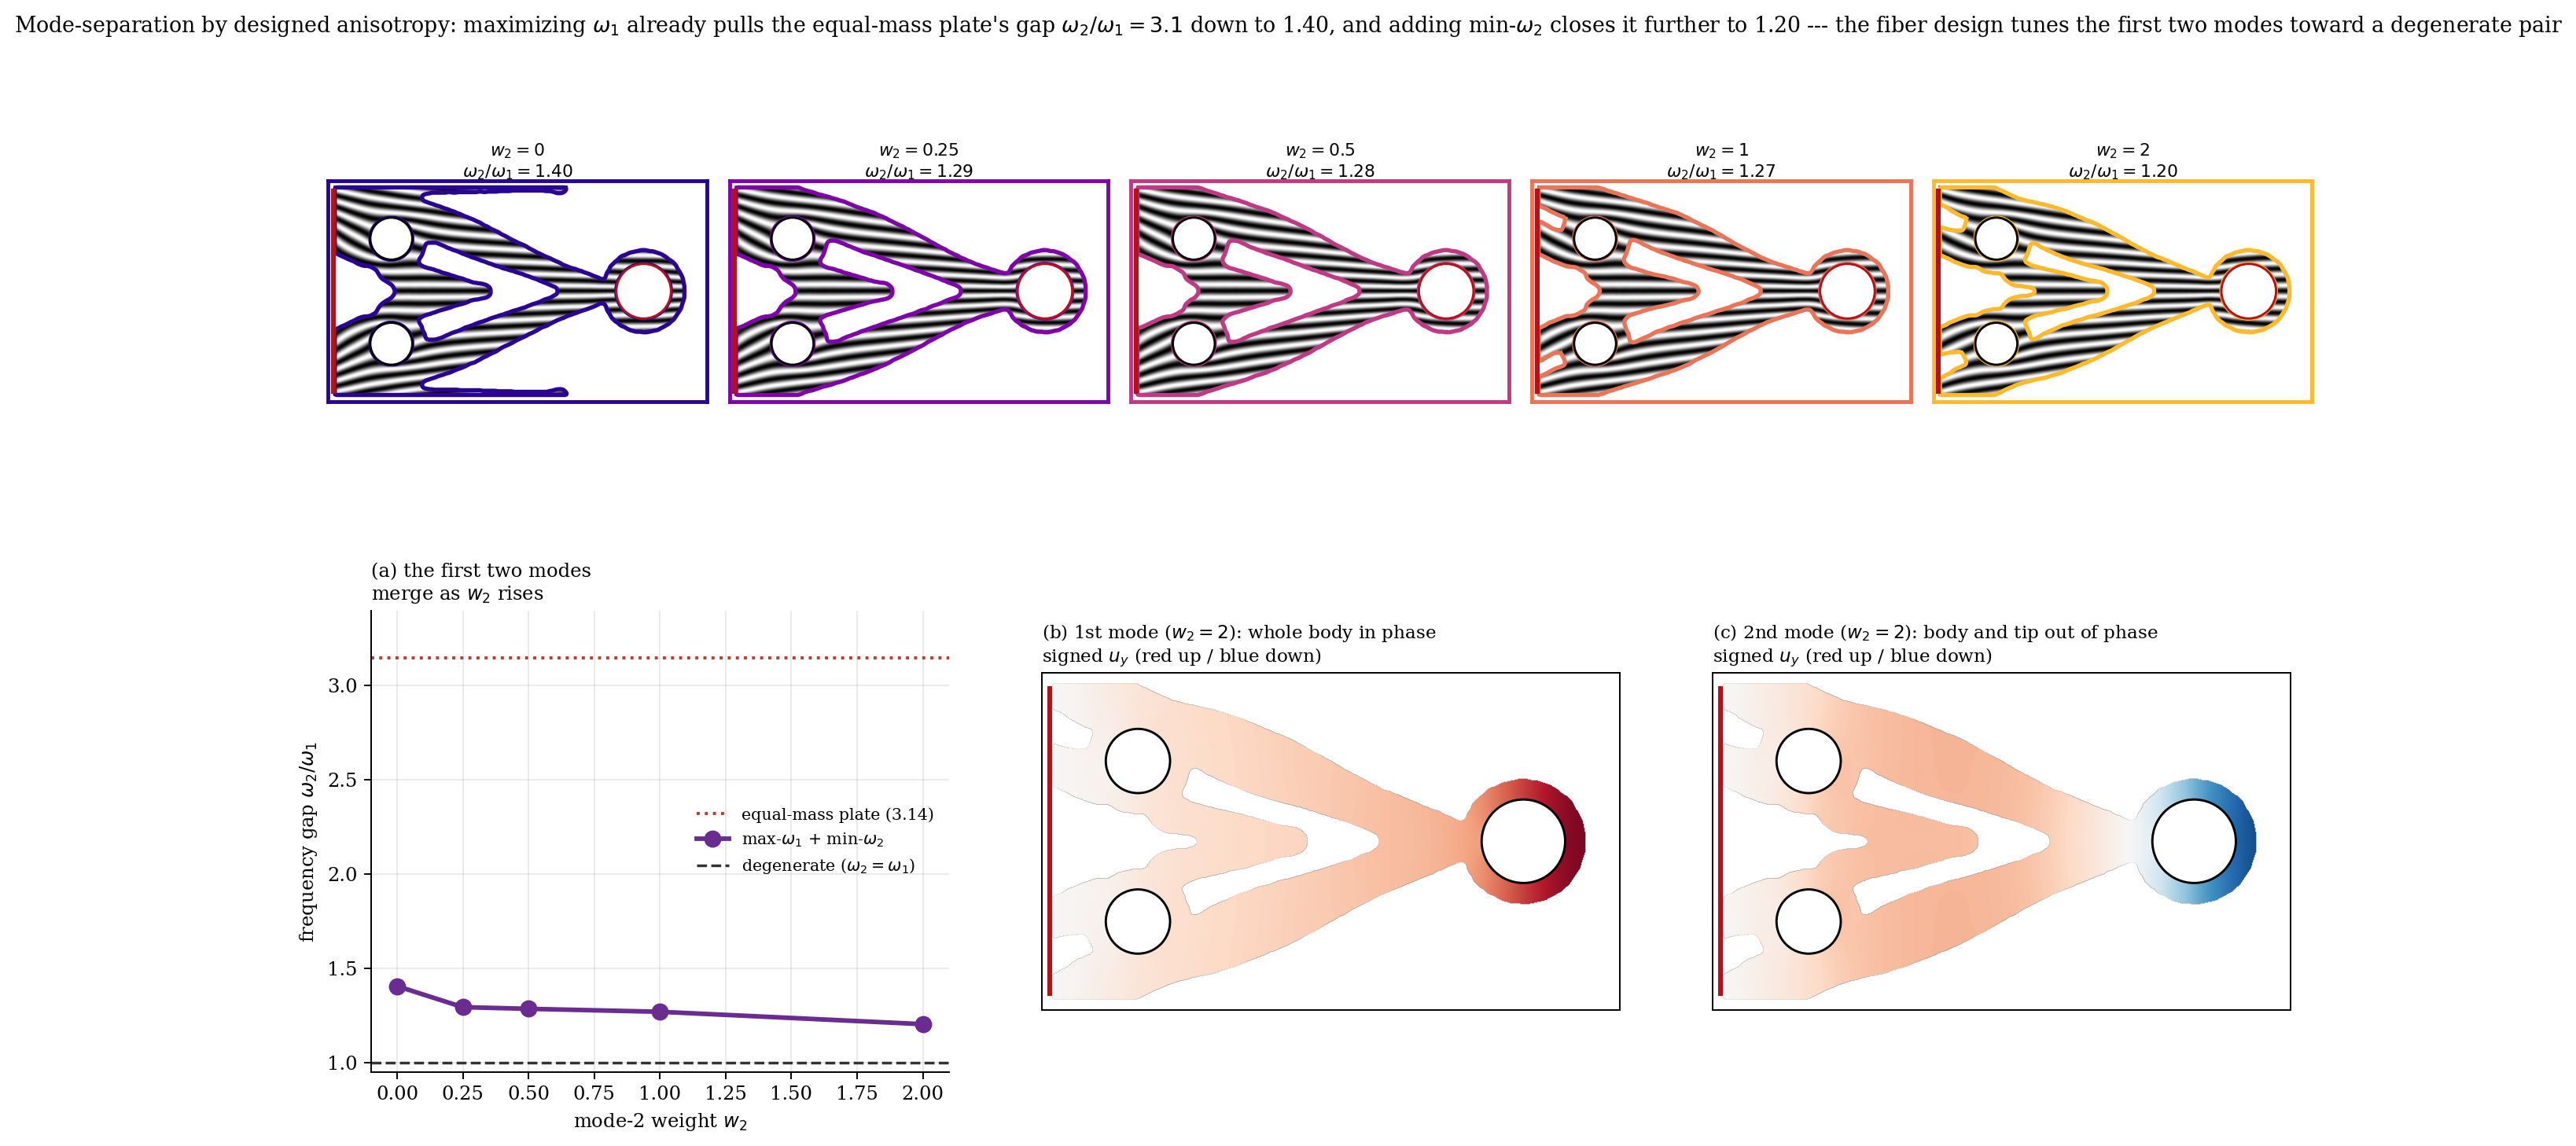
\includegraphics[width=0.98\textwidth]{figs/cfrp_bracket_mode2.png}}
  {\fbox{\parbox[c][32mm][c]{0.9\textwidth}{\centering\itshape
   figure pending: run in progress}}}
\caption{Mode separation by designed anisotropy: maximizing $\omega_1$ \emph{while
minimizing} $\omega_2$ drives the first two natural frequencies together at fixed mass.
\emph{Top:} topology and fiber tows as the mode-2 weight $w_2$ is raised. \emph{Bottom
left:} the gap $\omega_2/\omega_1$ collapses from ${\sim}4$ toward ${\sim}\BRTWOGAP$ ---
a near-degenerate fundamental pair. \emph{Bottom middle/right:} the first two mode shapes
of the most mode-merged design; the fiber field has tuned them to nearly coincide. This
is a purely anisotropic effect and a stringent check of the second-mode sensitivity.}
\label{fig:mode2}
\end{figure}

\section{Topological valley guiding, and what the mesh must resolve}
\label{sec:valley}
The orientation lever of \S\ref{sec:results} steers waves through a homogeneous
plate; the periodic cell of \S\ref{sec:meta} shapes a dispersion relation. A
third regime combines them: a \emph{topological} valley-Hall waveguide, in which
the orientation of a C$_3$ scatterer acts as a tunable Dirac mass and a domain
wall between mirror-partner orientations guides a kink mode. This section reports
that device, and --- because the result turns on it --- the discretization
requirement that makes it meaningful.

\subsection{The crystal and the protected window}
We use the scalar (antiplane-shear) problem on a triangular lattice
($\mathbf a_1=a(1,0)$, $\mathbf a_2=a(\tfrac12,\tfrac{\sqrt3}{2})$) with one
stiff equilateral-triangle rod per cell ($R=0.44a$, $\mu_f/\mu_m=100$). An
equilateral triangle is C$_{3\mathrm v}$; aligning its mirrors with the lattice's
gives a symmetry-protected Dirac cone at $K$, and rotating the rod by $\alpha$
breaks the mirror while preserving C$_3$, opening a valley gap with Dirac mass
$m\propto\cos(3\alpha)$. Mirror-partner domains ($\alpha$ and $60^\circ-\alpha$,
here $15^\circ|45^\circ$) carry opposite $m$, hence $|\Delta C_v|=1$, and their
interface hosts a kink mode.

Three independent calculations, all on \emph{rod-conforming} meshes
(\S\ref{sec:valley:mesh}), bound where that mode may be claimed as topological.
The complete bulk gap from the periodic cell
(\texttt{wavetopo/valley\_cell.py}, converged in Brillouin-zone sampling: the
band-2 maximum is stable to four decimals and the band-3 minimum moves by $0.019$
between $169$ and $1681$ $\mathbf k$-points) is
\begin{equation}
  \omega\in[\VGAPLO,\ \VGAPHI],\qquad \text{width }\VGAPW .
  \label{eq:vgap}
\end{equation}
The ribbon supercell with a $15^\circ|45^\circ$ wall carries a strongly
wall-localized branch spanning $\omega\approx6.5$ to $\VKINKHI$. The
\emph{protected window} is the intersection --- the wall branch lying inside the
complete gap:
\begin{equation}
  \omega\in[\VGAPLO,\ \VKINKHI].
  \label{eq:vprot}
\end{equation}

\paragraph{Guiding is broader than protection.} In the finite domain the wall
guides well over roughly $[7.05,7.85]$: the field hugs the wall and reaches a
probe at the far end, with wall confinement
$C=\int_{d<1}|u|^2/\int_{\rm int}|u|^2 = \VWCONF$ (against $\VWCONFB$ below the
gap). But confinement stays high to $\omega\approx7.85$, well \emph{above} the
complete gap edge $\VGAPHI$. Fields at $\omega=7.7$ confirm genuine, tightly
confined transport. It is nonetheless not topological: above $\VGAPHI$ bulk
states exist and the ribbon carries no wall branch, so what guides there is
conventional index contrast at the wall, not a gap-traversing kink mode. We
therefore restrict every protection claim to \eqref{eq:vprot} and report the
$7.6$--$7.85$ guiding separately as ordinary guiding. Distinguishing the two
requires the confinement measure: transmission to a probe registers energy that
arrived by \emph{any} route and reads high in both regimes, differing by only a
factor $\sim\!3$.

\subsection{Why the mesh must conform to the rods}
\label{sec:valley:mesh}
The natural finite-domain discretization --- mesh the rectangle, then assign each
element to rod or matrix by testing its centroid --- is the staircased
construction rejected for through-holes in \S\ref{sec:hole} and for the cloaked
void in \S\ref{sec:cloak}. Here it is not merely inaccurate but
\emph{disqualifying}, because the Dirac mass $m\propto\cos(3\alpha)$ \emph{is}
the C$_3$ symmetry breaking of the scatterer: a staircase that perturbs the rod's
threefold symmetry by an amount comparable to the intended mass perturbs the gap
itself.

The perturbation is not small. Painting rods onto a plain mesh at $h=0.09$ leaves
the \emph{mean} rod area correct to $0.09\%$ --- staircase errors average out over
$293$ rods, so a bulk fiber-fraction check does not detect the problem --- while
giving each individual rod a random area error and displacing its effective
centre by up to $\VRODOFF\%$ of $R$. Cutting the rods into the geometry instead
reproduces every rod exactly: per-rod area $0.251487$ with standard deviation
$2.2\times10^{-16}$ and centroid offset $3\times10^{-16}$.

Table~\ref{tab:vconv} shows the consequence. Sweeping wall transmission over
frequency at three resolutions, the conforming meshes agree to a factor
$\VCONVC$ and peak inside the gap \eqref{eq:vgap} at every resolution. The
painted meshes spread by a factor $\VCONVP$, and at the coarsest resolution their
peak falls at $\omega=8.0$, outside the gap altogether --- no guided band at all.
Painted meshes do converge toward the conforming answer, but slowly: at $h=0.06$
they are still a factor $\sim\!4$ low. The conforming construction is converged
at $h=0.12$, where the painted one is not converged at half that spacing.

\begin{table}[h]
\centering
\caption{Mesh-convergence of the guided band. $\bar T$ is the mean transmission
over the complete gap \eqref{eq:vgap}; $\omega_{\rm peak}$ is where transmission
is largest.}
\label{tab:vconv}
\begin{tabular}{llccc}
\toprule
mesh & $h$ & $\bar T$ (in gap) & $\omega_{\rm peak}$ & in gap? \\
\midrule
conforming & 0.12 & $1.97\times10^{-1}$ & 7.267 & yes \\
conforming & 0.09 & $3.71\times10^{-1}$ & 7.200 & yes \\
conforming & 0.06 & $2.99\times10^{-1}$ & 7.133 & yes \\
\midrule
painted    & 0.12 & $1.34\times10^{-4}$ & 8.000 & \textbf{no} \\
painted    & 0.09 & $1.38\times10^{-2}$ & 7.467 & yes \\
painted    & 0.06 & $7.88\times10^{-2}$ & 7.533 & yes \\
\bottomrule
\end{tabular}
\end{table}

\subsection{Robustness to wall defects}
Within the protected window we damage the wall and re-measure. At
$\omega=\VROMEGA$ on a conforming mesh, transmission falls from $\VRPRIS$
(pristine) to $\VRVAC\%$ of that value for a removed rod and $\VRDIS\%$ for a
cluster of rods rotated by $\pm12^\circ$, while all three remain more than three
orders of magnitude above the out-of-band floor (pristine contrast $\VRCON\times$).

Two qualifications keep this honest. First, this is degradation, not immunity: a
vacancy costs a factor $\sim\!5$. Valley-Hall protection suppresses
\emph{inter-valley} backscattering, and a vacancy is a sharp defect that supplies
exactly the large momentum transfer the mechanism does not forbid; the correct
claim is that the mode survives damage that would extinguish a resonant defect
line, not that it is immune. Second, a defect test is only meaningful if the
pristine transmission is well clear of the floor --- otherwise all three
configurations report noise and ``survives damage'' is vacuous. The driver
therefore refuses to run unless the pristine in-band/out-of-band contrast exceeds
a threshold. An earlier version of this study, on a painted mesh and at a
frequency read off a painted sweep, returned $4.2\times10^{-6}$,
$4.4\times10^{-6}$ and $1.2\times10^{-5}$ for the three configurations: all at
the deep-gap floor, and no conclusion about protection follows from them.

\appendix
\subsection{Exactly periodic phase on a unit cell}
\label{app:perphase}
On the metamaterial cell the construction above must be modified: no node may be
pinned, because $\psi$ is not periodic --- it must advance by a whole number of tow
cycles per lattice vector, or the tows will not join across the boundary. Split
\begin{equation}
  \Psi(\vx)=\psi_p(\vx)+n_x\frac{x}{a}+n_y\frac{y}{b},
  \qquad \psi_p\ \text{cell-periodic},\quad (n_x,n_y)\in\mathbb Z^2 .
  \label{eq:psisplit}
\end{equation}
The periodic part solves $\min_{\psi_p}\int_\Omega\lVert\nabla\psi_p-\mathbf
g/d\rVert^2$, which is \emph{diagonal} in the Fourier basis: with
$\psi_p=\sum_{\mathbf k}\hat\psi_{\mathbf k}e^{\ii\mathbf k\cdot\vx}$ and
$\nabla\mapsto\ii\mathbf k$, the normal equations
$\ii\mathbf k\cdot\overline{(\ii\mathbf k\hat\psi_{\mathbf k})}=
\ii\mathbf k\cdot\hat{\mathbf g}_{\mathbf k}/d$ give
\begin{equation}
  \boxed{\ \hat\psi_{\mathbf k}
  =-\ii\,\frac{\mathbf k\cdot\hat{\mathbf g}_{\mathbf k}}{d\,\lVert\mathbf k\rVert^2}
  \ \ (\mathbf k\neq\mathbf 0),\qquad \hat\psi_{\mathbf 0}=0\ }
  \label{eq:fftphase}
\end{equation}
--- the inverse divergence (Helmholtz projection) of $\mathbf g/d$, one FFT pair,
no linear solve. The $\mathbf k=\mathbf 0$ mode is precisely the part no periodic
function can carry, so the \emph{mean} gradient must be absorbed by the linear
term; matching it in the least-squares sense and rounding to the nearest
representable integer,
\begin{equation}
  n_x=\operatorname{round}\!\Bigl(\frac{a\,\langle g_x\rangle}{d}\Bigr),\qquad
  n_y=\operatorname{round}\!\Bigl(\frac{b\,\langle g_y\rangle}{d}\Bigr).
  \label{eq:towcount}
\end{equation}
The rounding is what buys exact periodicity: under $x\mapsto x+a$ the phase
advances by $n_x\in\mathbb Z$, so $\chi=\tfrac12+\tfrac12\cos(2\pi\Psi)$ is
\emph{unchanged}, and the tows join continuously across every cell boundary.

The price is a slight, uniform stretch of the pitch. Since rounding perturbs the
cycle count by at most $\tfrac12$ out of $n_{\rm tow}\approx a/d$ cycles, the
relative pitch error is bounded by
\begin{equation}
  \frac{|\Delta d|}{d}\ \le\ \frac{1}{2\,n_{\rm tow}}\ \approx\ \frac{d}{2a}.
  \label{eq:pitcherr}
\end{equation}
This is a second, independent reason to prefer a fine tow pitch in
\S\ref{sec:meta:sweep}: the coarsest level ($d=1/6$) can suffer up to $8.3\%$
pitch distortion in enforcing periodicity, the finest ($d=1/12$) at most $4.2\%$.
Exact periodicity and faithful pitch are competing goals, reconciled only by
taking $d\ll a$.

\subsection{Properties of the aggregation and symmetry operators}
\label{app:opprops}
\paragraph{KS bounds \eqref{eq:ksbound}.} Since every term of
$\sum_k e^{\rho v_k}$ is positive and one of them is $e^{\rho\max_k v_k}$,
$\sum_k e^{\rho v_k}\ge e^{\rho\max_k v_k}$, so
$\rho^{-1}\ln\sum_k e^{\rho v_k}\ge\max_k v_k$. Conversely every term is at most
$e^{\rho\max_k v_k}$, so $\sum_k e^{\rho v_k}\le N_ke^{\rho\max_k v_k}$ and
$\rho^{-1}\ln\sum_k e^{\rho v_k}\le\max_k v_k+\rho^{-1}\ln N_k$. Hence KS
\emph{over}-estimates a maximum and \emph{under}-estimates a minimum: the
aggregated bandwidth in \eqref{eq:flatobj} is an upper bound on the true sampled
bandwidth, and the aggregated gaps are lower bounds. Both errors are conservative
--- the optimizer is never rewarded for an artefact of the smoothing --- and both
vanish as $\rho^{-1}\ln N_k$. \qed
\subsection{Eigenvalue sensitivity for the Bloch metamaterial}
\label{sec:app:hf}
The band-structure objectives of \S\ref{sec:meta} are functions of the
eigenfrequencies $\omega_n(\mathbf k)$, so the optimizer needs
$\partial\omega_n/\partial p$ for each design variable $p$. Computing this by
finite differences would cost one extra eigensolve per variable per
$\mathbf k$-point --- thousands of eigensolves per iteration --- so we instead
use the analytic first-order perturbation result below, which delivers every
$\partial\lambda_n/\partial p$ from quantities \emph{already} computed by the
single eigensolve at that $\mathbf k$. This is the discrete counterpart of the
Hellmann--Feynman theorem of quantum mechanics (the energy derivative of a
Hamiltonian equals the expectation of the Hamiltonian's derivative in the
unperturbed state); the derivation makes precise why no eigenvector derivative
survives.

\paragraph{Setup.} At a fixed wavevector $\mathbf k$ the reduced problem
\eqref{eq:bloch} is the generalized Hermitian eigenproblem
\begin{equation}
  \mathbf K_r\,\bm\phi_n=\lambda_n\,\mathbf M_r\,\bm\phi_n,\qquad
  \lambda_n=\omega_n^2,\qquad
  \mathbf K_r=\mathbf K_r\HH,\ \ \mathbf M_r=\mathbf M_r\HH\succ0,
  \label{eq:app:geneig}
\end{equation}
with $\mathbf K_r,\mathbf M_r$ depending on the design $p\in\{z_e,\hat\theta_i\}$
through the assembled cell matrices. We assume $\lambda_n$ is a \emph{simple}
(non-degenerate) eigenvalue --- the caveat when it is not is discussed at the end
--- and fix the scale of the eigenvector by the $\mathbf M_r$-normalization
\begin{equation}
  \bm\phi_n\HH\mathbf M_r\bm\phi_n=1.
  \label{eq:app:norm}
\end{equation}
Write $(\cdot)'\equiv\partial(\cdot)/\partial p$. The matrices, the eigenvalue,
and the eigenvector all depend on $p$; the goal is $\lambda_n'$ alone.

\paragraph{Differentiate the eigen-relation.} Applying $\partial/\partial p$ to
\eqref{eq:app:geneig} by the product rule gives
\begin{equation}
  \mathbf K_r'\bm\phi_n+\mathbf K_r\bm\phi_n'
  =\lambda_n'\,\mathbf M_r\bm\phi_n
  +\lambda_n\mathbf M_r'\bm\phi_n
  +\lambda_n\mathbf M_r\bm\phi_n'.
  \label{eq:app:diff}
\end{equation}
This still contains the \emph{unknown} eigenvector derivative $\bm\phi_n'$, which
is expensive (it requires solving a singular system, or summing over all other
modes). The trick is to project it out. Left-multiply \eqref{eq:app:diff} by
$\bm\phi_n\HH$:
\begin{equation}
  \underbrace{\bm\phi_n\HH\mathbf K_r'\bm\phi_n}_{\text{(A)}}
  +\underbrace{\bm\phi_n\HH\mathbf K_r\bm\phi_n'}_{\text{(B)}}
  =\lambda_n'\underbrace{\bm\phi_n\HH\mathbf M_r\bm\phi_n}_{=1}
  +\lambda_n\underbrace{\bm\phi_n\HH\mathbf M_r'\bm\phi_n}_{\text{(C)}}
  +\lambda_n\underbrace{\bm\phi_n\HH\mathbf M_r\bm\phi_n'}_{\text{(D)}}.
  \label{eq:app:projected}
\end{equation}

\paragraph{Why the eigenvector-derivative terms cancel.} Consider the two terms
carrying $\bm\phi_n'$, namely (B) and (D). For (B), use that $\mathbf K_r$ is
Hermitian and $\bm\phi_n$ is its eigenvector: taking the conjugate transpose of
$\mathbf K_r\bm\phi_n=\lambda_n\mathbf M_r\bm\phi_n$ and using
$\mathbf K_r\HH=\mathbf K_r$, $\mathbf M_r\HH=\mathbf M_r$, $\lambda_n\in\mathbb
R$ (real, since the pencil is Hermitian-definite) gives the \emph{left}
eigen-relation
\begin{equation}
  \bm\phi_n\HH\mathbf K_r=\lambda_n\,\bm\phi_n\HH\mathbf M_r.
  \label{eq:app:left}
\end{equation}
Substituting \eqref{eq:app:left} into (B),
\[
  \text{(B)}=\bm\phi_n\HH\mathbf K_r\bm\phi_n'
  =\lambda_n\,\bm\phi_n\HH\mathbf M_r\bm\phi_n'
  =\lambda_n\,\text{(D)},
\]
so on the right-hand side the term $\lambda_n\cdot\text{(D)}$ is \emph{identical}
to (B) on the left, and the two cancel when \eqref{eq:app:projected} is
rearranged. The unknown $\bm\phi_n'$ has dropped out entirely --- this is the
crux, and it is exactly the discrete Hellmann--Feynman cancellation: the
first-order change of a normalized eigenvector is $\mathbf M_r$-orthogonal to the
mode itself, so it cannot change the Rayleigh quotient to first order. (Note we
did \emph{not} need $\partial/\partial p$ of the normalization
\eqref{eq:app:norm}; the cancellation is purely a consequence of the left
eigen-relation. Differentiating \eqref{eq:app:norm} gives the complementary fact
$2\Real(\bm\phi_n\HH\mathbf M_r\bm\phi_n')=-\bm\phi_n\HH\mathbf M_r'\bm\phi_n$,
which fixes the component of $\bm\phi_n'$ along $\bm\phi_n$ but is not needed
here.)

\paragraph{Result.} What remains of \eqref{eq:app:projected} is the
Hellmann--Feynman sensitivity
\begin{equation}
  \boxed{\;\frac{\partial\lambda_n}{\partial p}
  =\bm\phi_n\HH\Bigl(\frac{\partial\mathbf K_r}{\partial p}
  -\lambda_n\frac{\partial\mathbf M_r}{\partial p}\Bigr)\bm\phi_n\;}
  \tag{\ref{eq:eigsens}}
\end{equation}
and then $\partial\omega_n/\partial p=\partial\lambda_n/\partial p/(2\omega_n)$.
The formula has a clean physical reading: $\bm\phi_n\HH\mathbf K_r'\bm\phi_n$ is
the change in the mode's \emph{elastic (strain) energy} caused by the design
perturbation, and $\lambda_n\,\bm\phi_n\HH\mathbf M_r'\bm\phi_n$ the corresponding
change in its \emph{kinetic energy}; the eigenfrequency rises when the
perturbation stiffens the mode faster than it mass-loads it, and falls otherwise.
Everything on the right is available from the one eigenpair $(\lambda_n,
\bm\phi_n)$ already computed --- no extra solve, no eigenvector derivative.

\paragraph{Reduction to element energies.} The reduced matrices are congruence
transforms of the full-cell matrices, $\mathbf K_r=\mathbf T\HH\mathbf K\mathbf T$
and $\mathbf M_r=\mathbf T\HH\mathbf M\mathbf T$, with the Bloch reduction
$\mathbf T(\mathbf k)$ \emph{independent} of the design. Hence
$\mathbf K_r'=\mathbf T\HH\mathbf K'\mathbf T$ and likewise for $\mathbf M_r'$, and
\eqref{eq:eigsens} becomes a quadratic form in the full-space Bloch state
$\bm\psi_n=\mathbf T\bm\phi_n$:
\begin{equation}
  \frac{\partial\lambda_n}{\partial p}
  =\bm\psi_n\HH\frac{\partial\mathbf K}{\partial p}\bm\psi_n
  -\lambda_n\,\bm\psi_n\HH\frac{\partial\mathbf M}{\partial p}\bm\psi_n.
\end{equation}
Because $\mathbf K=\sum_e\mathbf k_e$ and $\mathbf M=\sum_e\mathbf m_e$ are
element-assembled and each element depends on the design only locally, both
quadratic forms collapse to sums of \emph{element energies} of $\bm\psi_n$. For
an orientation variable $\hat\theta_i$, only $\mathbf K$ depends on it (through
$\mathbf k_f(\theta)$), and the dependence passes through the CS-RBF map
$\theta=\hat{\bm\Phi}\hat{\bm\theta}$, so by the chain rule
\begin{equation}
  \frac{\partial\lambda_n}{\partial\hat\theta_i}
  =\sum_e\hat\Phi_{ei}\,z_e^{\,p}\,
  \bm\psi_{n,e}\HH\frac{\partial\mathbf k_f}{\partial\theta}(\theta_e)\,
  \bm\psi_{n,e},
\end{equation}
with $\partial\mathbf k_f/\partial\theta$ the exact Fourier derivative
\eqref{eq:dDf}. For a density variable $z_e$, the two-phase SIMP interpolation
gives $\partial\mathbf k_e/\partial z_e=p\,z_e^{p-1}(\mathbf k_f-\mathbf k_m)$ and
$\partial\mathbf m_e/\partial z_e=(\rho_f-\rho_m)\mathbf m_e^0$, so
\begin{equation}
  \frac{\partial\lambda_n}{\partial z_e}
  =p\,z_e^{p-1}\,\bm\psi_{n,e}\HH(\mathbf k_f-\mathbf k_m)\bm\psi_{n,e}
  -\lambda_n(\rho_f-\rho_m)\,\bm\psi_{n,e}\HH\mathbf m_e^0\bm\psi_{n,e}.
\end{equation}
These per-band, per-$\mathbf k$ gradients are then combined by the smooth KS
extrema of \eqref{eq:flatobj} (\texttt{flatband\_opt.py}) and finite-difference
verified to $\sim\!10^{-6}$.

\paragraph{Caveat: degenerate eigenvalues.} The cancellation above assumed
$\lambda_n$ simple, so that $\bm\phi_n$ is defined up to a phase and (B)$=\lambda_n
\cdot$(D) holds for \emph{that} eigenvector. At a degenerate eigenvalue --- e.g.\
the four-fold $\Gamma$-point degeneracy of a symmetric cell --- the eigenvectors
within the degenerate subspace are only defined up to a unitary mixing, the map
$p\mapsto\lambda_n(p)$ is generally not differentiable (only directionally so),
and \eqref{eq:eigsens} evaluated on an arbitrary basis of the subspace disagrees
with finite differences by order one. This is not a defect of the formula but of
the question: one must instead diagonalize the $2\times2$ (or $d\times d$)
restriction of $\mathbf K_r'-\lambda_n\mathbf M_r'$ onto the degenerate subspace
to get the (one-sided) sensitivities of the split branches. In practice we sidestep
this by starting the optimizer from a deliberately symmetry-broken cell, where all
bands of interest are simple; \S\ref{sec:multifunc} records the failure mode when
this is neglected.

\subsection{Eigenvalue sensitivity for the finite bracket}
\label{app:modalsens}
The bracket (\S\ref{sec:bracket}) maximizes the fundamental eigenvalue
$\lambda_1=\omega_1^2$ of the clamped generalized problem
$\mathbf K(z,\theta)\,\bm\phi=\lambda\,\mathbf M(z)\,\bm\phi$, with $\bm\phi$
mass-normalized, $\bm\phi\T\mathbf M\bm\phi=1$. For a simple eigenvalue the
Rayleigh-quotient derivative w.r.t.\ any design parameter $p$ is
\begin{equation}
  \frac{\partial\lambda_1}{\partial p}
   =\bm\phi\T\!\Bigl(\frac{\partial\mathbf K}{\partial p}
     -\lambda_1\frac{\partial\mathbf M}{\partial p}\Bigr)\bm\phi ,
  \label{eq:eigsens_bracket}
\end{equation}
the eigenvector's own variation dropping out at first order. Orientation leaves the
mass untouched ($\partial\mathbf M/\partial\theta=0$), so with the five-term
decomposition \eqref{eq:kffourier},
$\partial\lambda_1/\partial\theta_e
  =w(z_e)\,\bm\phi_e\T(\partial\mathbf k_f/\partial\theta_e)\bm\phi_e$.
Density moves both operators, but \emph{differently}: the stiffness is SIMP-penalized,
$\mathbf k_e=w(z_e)\mathbf k_f+(1-w(z_e))\mathbf k_m$ with $w(z)=z^{p}$, while the
element mass is \emph{linear} in the density,
$\mathbf m_e=[z_e\rho_f+(1-z_e)\rho_m]\,\mathbf m_0$ --- the standard modified-SIMP
mass interpolation that keeps low-density regions from carrying spurious low-frequency
modes. Hence
\begin{equation}
  \frac{\partial\lambda_1}{\partial z_e}
   =\underbrace{w'(z_e)\,\bm\phi_e\T(\mathbf k_f-\mathbf k_m)\bm\phi_e}
     _{\text{stiffen where the mode strains}}
   \;-\;\underbrace{\lambda_1(\rho_f-\rho_m)\,\bm\phi_e\T\mathbf m_0\bm\phi_e}
     _{\text{remove mass at the antinodes}} .
  \label{eq:eigsens_z}
\end{equation}
The second, negative term is the counterintuitive one and is the whole point of the
example: $\bm\phi_e\T\mathbf m_0\bm\phi_e$ is the element's kinetic energy in the mode,
so \emph{removing} material from the mode's antinodes \emph{raises} $\lambda_1$. At a
fixed mass budget the optimizer therefore moves material toward the strained regions
and away from the antinodes, lifting $\omega_1$ far more than a uniform stiffening
would. Both \eqref{eq:eigsens_bracket}--\eqref{eq:eigsens_z} pass the
finite-difference check to a gradient-normalized $\lesssim10^{-6}$, and the $\theta$
part isotropy-annihilates ($\partial\lambda_1/\partial\theta\to0$ as
$\mathbf Q_f\to$ isotropic, Remark~\ref{rem:iso}) to $O(10^{-18})$.

\subsection{p-norm stress sensitivity}
\label{app:stresssens}
The bracket's stress objective is the peak von Mises stress under the tip load,
smoothed by the p-norm surrogate
\begin{equation}
  \Sigma_p=\Bigl(\sum_e \tfrac{A_e}{\sum_k A_k}\,\tilde\sigma_e^{\,p}\Bigr)^{1/p},
  \qquad
  \tilde\sigma_e=z_e^{\,q}\sqrt{\bm\sigma_e\T\mathbf V\bm\sigma_e},\quad
  \bm\sigma_e=\mathbf D_f(\theta_e)\,\mathbf B_e\mathbf u_e ,
\end{equation}
where $\mathbf u$ solves the static problem $\mathbf K(z,\theta)\mathbf u=\mathbf F_s$,
$\mathbf V$ is the plane-stress von Mises matrix (so
$\bm\sigma\T\mathbf V\bm\sigma=\sigma_{xx}^2-\sigma_{xx}\sigma_{yy}+\sigma_{yy}^2
+3\tau_{xy}^2$), and $z_e^{\,q}$ ($q=\tfrac12$) is a qp-relaxation that stops void
elements from carrying spurious stress. The design derivative has an explicit part ---
the element stress depends on $z$ through the qp factor and on $\theta$ through
$\mathbf D_f$ --- and an implicit part through $\mathbf u$; the latter is a single
adjoint solve reusing the static factorization,
$\mathbf K\bm\mu=\partial\Sigma_p/\partial\mathbf u$, after which
$\partial\Sigma_p/\partial p=\partial\Sigma_p/\partial p|_{\rm expl}
-\bm\mu\T(\partial\mathbf K/\partial p)\,\mathbf u$ for $p\in\{z,\theta\}$
($\mathbf K$ symmetric). The $z^{q-1}$ in the explicit qp term is regular once carried
by the p-norm weight (whose factor $\tilde\sigma_e^{\,p-1}\!\to0$ as $z_e\to0$); both
$\partial\Sigma_p/\partial z$ and $\partial\Sigma_p/\partial\theta$ pass the
finite-difference check to a gradient-normalized $\lesssim10^{-7}$.


\begin{thebibliography}{1}
\bibitem{wong2025}
J.~Wong, E.~D.~Sanders, D.~W.~Rosen,
\emph{Toolpath-integrated topology optimization for design of additively
manufactured fiber-reinforced structures considering limits on fiber curvature},
Composite Structures (2025). Reference implementation and manufacturing
constraints adapted here to elastic wave control; local file
\texttt{toolpathtocfrp-comstr2025.pdf}.
\bibitem{norris2008}
A.~N.~Norris, \emph{Acoustic cloaking theory}, Proc.\ R.\ Soc.\ A \textbf{464}
(2008) 2411--2434. The transformation cloak requires anisotropic material whose
properties are \emph{singular} at the inner surface (infinite inertia for isotropic
stiffness, or a pentamode with diverging anisotropy) --- the physical origin of the
fiber-curvature singularity we compare against in \S\ref{sec:cloak}.
\bibitem{pendry2006}
J.~B.~Pendry, D.~Schurig, D.~R.~Smith, \emph{Controlling electromagnetic fields},
Science \textbf{312} (2006) 1780--1782. Source of the radial cloak transformation
$r'=R_V+r\,(R_{\rm des}-R_V)/R_{\rm des}$ whose fiber image we evaluate.
\end{thebibliography}
\end{document}
